\documentclass[type=master]{thuthesis}
% 选项:
%   type=[bachelor|master|doctor|postdoctor], % 必选
%   secret,                                   % 可选
%   pifootnote,                               % 可选(建议打开)
%   openany|openright,                        % 可选,基本不用
%   arial,                                    % 可选,基本不用
%   arialtoc,                                 % 可选,基本不用
%   arialtitle                                % 可选,基本不用

% 所有其它可能用到的包都统一放到这里了,可以根据自己的实际添加或者删除。
\usepackage{thuthesis}

% 定义所有的图片文件在 figures 子目录下
\graphicspath{{figures/}}

% 可以在这里修改配置文件中的定义。导言区可以使用中文。
% \def\myname{薛瑞尼}

\begin{document}

%%% 封面部分
\frontmatter
\thusetup{
  %******************************
  % 注意:
  %   1. 配置里面不要出现空行
  %   2. 不需要的配置信息可以删除
  %******************************
  %
  %=====
  % 秘级
  %=====
  %secretlevel={秘密},
  %secretyear={10},
  %
  %=========
  % 中文信息
  %=========
  ctitle={基于深度神经网络的多尺度故障诊断方法研究},
  cdegree={工学硕士},
  cdepartment={自动化系},
  cmajor={控制科学与工程},
  cauthor={李亮民},
  csupervisor={李志恒副教授},
  %cassosupervisor={陈文光教授}, % 副指导老师
  %ccosupervisor={某某某教授}, % 联合指导老师
  % 日期自动使用当前时间,若需指定按如下方式修改:
  % cdate={超新星纪元},
  %
  % 博士后专有部分
  %cfirstdiscipline={计算机科学与技术},
  %cseconddiscipline={系统结构},
  %postdoctordate={2009年7月——2011年7月},
  %id={编号}, % 可以留空: id={},
  %udc={UDC}, % 可以留空
  %catalognumber={分类号}, % 可以留空
  %
  %=========
  % 英文信息
  %=========
  etitle={Research on Multi-scale Fault Diagnosis Method Based on Deep Neural Network},
  % 这块比较复杂,需要分情况讨论:
  % 1. 学术型硕士
  %    edegree:必须为Master of Arts或Master of Science(注意大小写)
  %             “哲学、文学、历史学、法学、教育学、艺术学门类,公共管理学科
  %              填写Master of Arts,其它填写Master of Science”
  %    emajor:“获得一级学科授权的学科填写一级学科名称,其它填写二级学科名称”
  % 2. 专业型硕士
  %    edegree:“填写专业学位英文名称全称”
  %    emajor:“工程硕士填写工程领域,其它专业学位不填写此项”
  % 3. 学术型博士
  %    edegree:Doctor of Philosophy(注意大小写)
  %    emajor:“获得一级学科授权的学科填写一级学科名称,其它填写二级学科名称”
  % 4. 专业型博士
  %    edegree:“填写专业学位英文名称全称”
  %    emajor:不填写此项
  edegree={Master of Science},
  emajor={Control Science and Engineering},
  eauthor={Li Liangmin},
  esupervisor={Associate Professor Li Zhiheng},
  %eassosupervisor={Chen Wenguang},
  % 日期自动生成,若需指定按如下方式修改:
  % edate={December, 2005}
  %
  % 关键词用“英文逗号”分割
  ckeywords={故障诊断, 机器学习, 神经网络, 多尺度, 特征提取},
  ekeywords={Fault Diagnosis, Machine Learning, Neural Network, Multi-scale, Feature Extraction}
}

% 定义中英文摘要和关键字
\begin{cabstract}
  论文的摘要是对论文研究内容和成果的高度概括。摘要应对论文所研究的问题及其研究目
  的进行描述,对研究方法和过程进行简单介绍,对研究成果和所得结论进行概括。摘要应
  具有独立性和自明性,其内容应包含与论文全文同等量的主要信息。使读者即使不阅读全
  文,通过摘要就能了解论文的总体内容和主要成果。

  论文摘要的书写应力求精确、简明。切忌写成对论文书写内容进行提要的形式,尤其要避
  免“第 1 章……;第 2 章……;……”这种或类似的陈述方式。

  本文介绍清华大学论文模板 \thuthesis{} 的使用方法。本模板符合学校的本科、硕士、
  博士论文格式要求。

  本文的创新点主要有:
  \begin{itemize}
    \item 用例子来解释模板的使用方法;
    \item 用废话来填充无关紧要的部分;
    \item 一边学习摸索一边编写新代码。
  \end{itemize}

  关键词是为了文献标引工作、用以表示全文主要内容信息的单词或术语。关键词不超过 5
  个,每个关键词中间用分号分隔。(模板作者注:关键词分隔符不用考虑,模板会自动处
  理。英文关键词同理。)
\end{cabstract}

% 如果习惯关键字跟在摘要文字后面,可以用直接命令来设置,如下:
% \ckeywords{\TeX, \LaTeX, CJK, 模板, 论文}

\begin{eabstract}
   An abstract of a dissertation is a summary and extraction of research work
   and contributions. Included in an abstract should be description of research
   topic and research objective, brief introduction to methodology and research
   process, and summarization of conclusion and contributions of the
   research. An abstract should be characterized by independence and clarity and
   carry identical information with the dissertation. It should be such that the
   general idea and major contributions of the dissertation are conveyed without
   reading the dissertation.

   An abstract should be concise and to the point. It is a misunderstanding to
   make an abstract an outline of the dissertation and words ``the first
   chapter'', ``the second chapter'' and the like should be avoided in the
   abstract.

   Key words are terms used in a dissertation for indexing, reflecting core
   information of the dissertation. An abstract may contain a maximum of 5 key
   words, with semi-colons used in between to separate one another.
\end{eabstract}

% \ekeywords{\TeX, \LaTeX, CJK, template, thesis}

% 如果使用授权说明扫描页,将可选参数中指定为扫描得到的 PDF 文件名,例如:
% \makecover[scan-auth.pdf]
\makecover

%% 目录
\tableofcontents

%% 符号对照表
\begin{denotation}[3cm]
\item[HPC] 高性能计算 (High Performance Computing)
\item[cluster] 集群
\item[Itanium] 安腾
\item[SMP] 对称多处理
\item[API] 应用程序编程接口
\item[PI] 聚酰亚胺
\item[MPI] 聚酰亚胺模型化合物,N-苯基邻苯酰亚胺
\item[PBI] 聚苯并咪唑
\item[MPBI] 聚苯并咪唑模型化合物,N-苯基苯并咪唑
\item[PY] 聚吡咙
\item[PMDA-BDA]	均苯四酸二酐与联苯四胺合成的聚吡咙薄膜
\item[$\Delta G$] 活化自由能 (Activation Free Energy)
\item[$\chi$] 传输系数 (Transmission Coefficient)
\item[$E$] 能量
\item[$m$] 质量
\item[$c$] 光速
\item[$P$] 概率
\item[$T$] 时间
\item[$v$] 速度
\item[劝学] 君子曰:学不可以已。青,取之于蓝,而青于蓝;冰,水为之,而寒于水。木
  直中绳。輮以为轮,其曲中规。虽有槁暴,不复挺者,輮使之然也。故木受绳则直,金就
  砺则利,君子博学而日参省乎己,则知明而行无过矣。吾尝终日而思矣,不如须臾之所学
  也;吾尝跂而望矣,不如登高之博见也。登高而招,臂非加长也,而见者远;顺风而呼,
  声非加疾也,而闻者彰。假舆马者,非利足也,而致千里;假舟楫者,非能水也,而绝江
  河,君子生非异也,善假于物也。积土成山,风雨兴焉;积水成渊,蛟龙生焉;积善成德,
  而神明自得,圣心备焉。故不积跬步,无以至千里;不积小流,无以成江海。骐骥一跃,
  不能十步;驽马十驾,功在不舍。锲而舍之,朽木不折;锲而不舍,金石可镂。蚓无爪牙
  之利,筋骨之强,上食埃土,下饮黄泉,用心一也。蟹六跪而二螯,非蛇鳝之穴无可寄托
  者,用心躁也。—— 荀况
\end{denotation}



%%% 正文部分
\mainmatter
\chapter{带 English 的标题}
\label{cha:intro}

这是 \thuthesis{} 的示例文档,基本上覆盖了模板中所有格式的设置。建议大家在使用模
板之前,除了阅读《\thuthesis{}用户手册》,这个示例文档也最好能看一看。

小老鼠偷吃热凉粉;短长虫环绕矮高粱\footnote{韩愈(768-824),字退之,河南河阳(
  今河南孟县)人,自称郡望昌黎,世称韩昌黎。幼孤贫刻苦好学,德宗贞元八年进士。曾
  任监察御史,因上疏请免关中赋役,贬为阳山县令。后随宰相裴度平定淮西迁刑部侍郎,
  又因上表谏迎佛骨,贬潮州刺史。做过吏部侍郎,死谥文公,故世称韩吏部、韩文公。是
  唐代古文运动领袖,与柳宗元合称韩柳。诗力求险怪新奇,雄浑重气势。}。


\section{封面相关}
封面的例子请参看 cover.tex。主要符号表参看 denation.tex,附录和个人简历分别参看 appendix01.tex
和 resume.tex。里面的命令都很只管,一看即会\footnote{你说还是看不懂?怎么会呢?}。

\section{字体命令}
\label{sec:first}

苏轼(1037-1101),北宋文学家、书画家。字子瞻,号东坡居士,眉州眉山(今属四川)人
。苏洵子。嘉佑进士。神宗时曾任祠部员外郎,因反对王安石新法而求外职,任杭州通判,
知密州、徐州、湖州。后以作诗“谤讪朝廷”罪贬黄州。哲宗时任翰林学士,曾出知杭州、
颖州等,官至礼部尚书。后又贬谪惠州、儋州。北还后第二年病死常州。南宋时追谥文忠。
与父洵弟辙,合称“三苏”。在政治上属于旧党,但也有改革弊政的要求。其文汪洋恣肆,
明白畅达,为“唐宋八大家”之一。  其诗清新豪健,善用夸张比喻,在艺术表现方面独具
风格。少数诗篇也能反映民间疾苦,指责统治者的奢侈骄纵。词开豪放一派,对后代很有影
响。《念奴娇·赤壁怀古》、《水调歌头·丙辰中秋》传诵甚广。

{\kaishu 坡仙擅长行书、楷书,取法李邕、徐浩、颜真卿、杨凝式,而能自创新意。用笔丰腴
  跌宕,有天真烂漫之趣。与蔡襄、黄庭坚、米芾并称“宋四家”。能画竹,学文同,也喜
  作枯木怪石。论画主张“神似”,认为“论画以形似,见与儿童邻”;高度评价“诗中有
  画,画中有诗”的艺术造诣。诗文有《东坡七集》等。存世书迹有《答谢民师论文帖》、
  《祭黄几道文》、《前赤壁赋》、《黄州寒食诗帖》等。  画迹有《枯木怪石图》、《
  竹石图》等。}

{\fangsong 易与天地准,故能弥纶天地之道。仰以观於天文,俯以察於地理,是故知幽明之故。原
  始反终,故知死生之说。精气为物,游魂为变,是故知鬼神之情状。与天地相似,故不违。
  知周乎万物,而道济天下,故不过。旁行而不流,乐天知命,故不忧。安土敦乎仁,故
  能爱。范围天地之化而不过,曲成万物而不遗,通乎昼夜之道而知,故神无方而易无体。}

% 非本科生一般用不到幼圆与隶书字体。需要的同学请查看 ctex 文档。
{\ifcsname youyuan\endcsname\youyuan\else[无 \cs{youyuan} 字体。]\fi 有天地,然后
  万物生焉。盈天地之间者,唯万物,故受之以屯;屯者盈也,屯者物之始生也。物生必蒙,
  故受之以蒙;蒙者蒙也,物之穉也。物穉不可不养也,故受之以需;需者饮食之道也。饮
  食必有讼,故受之以讼。讼必有众起,故受之以师;师者众也。众必有所比,故受之以比;
  比者比也。比必有所畜也,故受之以小畜。物畜然后有礼,故受之以履。}

{\heiti 履而泰,然后安,故受之以泰;泰者通也。物不可以终通,故受之以否。物不可以终
  否,故受之以同人。与人同者,物必归焉,故受之以大有。有大者不可以盈,故受之以谦。
  有大而能谦,必豫,故受之以豫。豫必有随,故受之以随。以喜随人者,必有事,故受
  之以蛊;蛊者事也。}

{\ifcsname lishu\endcsname\lishu\else[无 \cs{lishu} 字体。]\fi 有事而后可大,故受
  之以临;临者大也。物大然后可观,故受之以观。可观而后有所合,故受之以噬嗑;嗑者
  合也。物不可以苟合而已,故受之以贲;贲者饰也。致饰然后亨,则尽矣,故受之以剥;
  剥者剥也。物不可以终尽,剥穷上反下,故受之以复。复则不妄矣,故受之以无妄。}

{\songti 有无妄然后可畜,故受之以大畜。物畜然后可养,故受之以颐;颐者养也。不养则不
  可动,故受之以大过。物不可以终过,故受之以坎;坎者陷也。陷必有所丽,故受之以
  离;离者丽也。}

\section{表格样本}
\label{chap1:sample:table} 

\subsection{基本表格}
\label{sec:basictable}

模板中关于表格的宏包有三个: \pkg{booktabs}、\pkg{array} 和
\pkg{longtabular},命令有一个 \cs{hlinewd}。三线表可以用 \pkg{booktabs}
提供的 \cs{toprule}、\cs{midrule} 和 \cs{bottomrule}。它们与
\pkg{longtable} 能很好的配合使用。如果表格比较简单的话可以直接用命令
\cs{hlinewd}\marg{width} 控制。
\begin{table}[htb]
  \centering
  \begin{minipage}[t]{0.8\linewidth} % 如果想在表格中使用脚注,minipage是个不错的办法
  \caption[模板文件]{模板文件。如果表格的标题很长,那么在表格索引中就会很不美
    观,所以要像 chapter 那样在前面用中括号写一个简短的标题。这个标题会出现在索
    引中。}
  \label{tab:template-files}
    \begin{tabularx}{\linewidth}{lX}
      \toprule[1.5pt]
      {\heiti 文件名} & {\heiti 描述} \\\midrule[1pt]
      thuthesis.ins & \LaTeX{} 安装文件,\textsc{DocStrip}\footnote{表格中的脚注} \\
      thuthesis.dtx & 所有的一切都在这里面\footnote{再来一个}。\\
      thuthesis.cls & 模板类文件。\\
      thuthesis.cfg & 模板配置文。cls 和 cfg 由前两个文件生成。\\
      thuthesis.bst    & 参考文献 BIB\TeX\ 样式文件。\\
      thuthesis.sty   & 常用的包和命令写在这里,减轻主文件的负担。\\
      \bottomrule[1.5pt]
    \end{tabularx}
  \end{minipage}
\end{table}

首先来看一个最简单的表格。表 \ref{tab:template-files} 列举了本模板主要文件及其功
能。请大家注意三线表中各条线对应的命令。这个例子还展示了如何在表格中正确使用脚注。
由于 \LaTeX{} 本身不支持在表格中使用 \cs{footnote},所以我们不得不将表格放在
小页中,而且最好将表格的宽度设置为小页的宽度,这样脚注看起来才更美观。

\subsection{复杂表格}
\label{sec:complicatedtable}

我们经常会在表格下方标注数据来源,或者对表格里面的条目进行解释。前面的脚注是一种
不错的方法,如果不喜欢脚注,可以在表格后面写注释,比如表~\ref{tab:tabexamp1}。
\begin{table}[htbp]
  \centering
  \caption{复杂表格示例 1}
  \label{tab:tabexamp1}
  \begin{minipage}[t]{0.8\textwidth} 
    \begin{tabularx}{\linewidth}{|l|X|X|X|X|}
      \hline
 \multirow{2}*{\diagbox[width=5em]{x}{y}} & \multicolumn{2}{c|}{First Half} & \multicolumn{2}{c|}{Second Half}\\\cline{2-5}
      & 1st Qtr &2nd Qtr&3rd Qtr&4th Qtr \\ \hline
      East$^{*}$ &   20.4&   27.4&   90&     20.4 \\
      West$^{**}$ &   30.6 &   38.6 &   34.6 &  31.6 \\ \hline
    \end{tabularx}\\[2pt]
    \footnotesize 注:数据来源《\thuthesis{} 使用手册》。\\
    *:东部\\
    **:西部
  \end{minipage}
\end{table}

此外,表~\ref{tab:tabexamp1} 同时还演示了另外两个功能:1)通过 \pkg{tabularx} 的
 \texttt{|X|} 扩展实现表格自动放大;2)通过命令 \cs{diagbox} 在表头部分
插入反斜线。

为了使我们的例子更接近实际情况,我会在必要的时候插入一些“无关”文字,以免太多图
表同时出现,导致排版效果不太理想。第一个出场的当然是我的最爱:风流潇洒、骏马绝尘、
健笔凌云的{\heiti 李太白}了。

李白,字太白,陇西成纪人。凉武昭王暠九世孙。或曰山东人,或曰蜀人。白少有逸才,志
气宏放,飘然有超世之心。初隐岷山,益州长史苏颋见而异之,曰:“是子天才英特,可比
相如。”天宝初,至长安,往见贺知章。知章见其文,叹曰:“子谪仙人也。”言于明皇,
召见金銮殿,奏颂一篇。帝赐食,亲为调羹,有诏供奉翰林。白犹与酒徒饮于市,帝坐沉香
亭子,意有所感,欲得白为乐章,召入,而白已醉。左右以水颒面,稍解,援笔成文,婉丽
精切。帝爱其才,数宴见。白常侍帝,醉,使高力士脱靴。力士素贵,耻之,摘其诗以激杨
贵妃。帝欲官白,妃辄沮止。白自知不为亲近所容,恳求还山。帝赐金放还。乃浪迹江湖,
终日沉饮。永王璘都督江陵,辟为僚佐。璘谋乱,兵败,白坐长流夜郎,会赦得还。族人阳
冰为当涂令,白往依之。代宗立,以左拾遗召,而白已卒。文宗时,诏以白歌诗、裴旻剑舞、
张旭草书为三绝云。集三十卷。今编诗二十五卷。\hfill —— 《全唐诗》诗人小传

浮动体的并排放置一般有两种情况:1)二者没有关系,为两个独立的浮动体;2)二者隶属
于同一个浮动体。对表格来说并排表格既可以像图~\ref{tab:parallel1}、图~\ref{tab:parallel2} 
使用小页环境,也可以如图~\ref{tab:subtable} 使用子表格来做。图的例子参见第~\ref{sec:multifig} 节。

\begin{table}[htbp]
\noindent\begin{minipage}{0.5\textwidth}
\centering
\caption{第一个并排子表格}
\label{tab:parallel1}
\begin{tabular}{p{2cm}p{2cm}}
\toprule[1.5pt]
111 & 222 \\\midrule[1pt]
222 & 333 \\\bottomrule[1.5pt]
\end{tabular}
\end{minipage}%
\begin{minipage}{0.5\textwidth}
\centering
\caption{第二个并排子表格}
\label{tab:parallel2}
\begin{tabular}{p{2cm}p{2cm}}
\toprule[1.5pt]
111 & 222 \\\midrule[1pt]
222 & 333 \\\bottomrule[1.5pt]
\end{tabular}
\end{minipage}
\end{table}

然后就是忧国忧民,诗家楷模杜工部了。杜甫,字子美,其先襄阳人,曾祖依艺为巩令,因
居巩。甫天宝初应进士,不第。后献《三大礼赋》,明皇奇之,召试文章,授京兆府兵曹参
军。安禄山陷京师,肃宗即位灵武,甫自贼中遁赴行在,拜左拾遗。以论救房琯,出为华州
司功参军。关辅饥乱,寓居同州同谷县,身自负薪采梠,餔糒不给。久之,召补京兆府功曹,
道阻不赴。严武镇成都,奏为参谋、检校工部员外郎,赐绯。武与甫世旧,待遇甚厚。乃于
成都浣花里种竹植树,枕江结庐,纵酒啸歌其中。武卒,甫无所依,乃之东蜀就高適。既至
而適卒。是岁,蜀帅相攻杀,蜀大扰。甫携家避乱荆楚,扁舟下峡,未维舟而江陵亦乱。乃
溯沿湘流,游衡山,寓居耒阳。卒年五十九。元和中,归葬偃师首阳山,元稹志其墓。天宝
间,甫与李白齐名,时称李杜。然元稹之言曰:“李白壮浪纵恣,摆去拘束,诚亦差肩子美
矣。至若铺陈终始,排比声韵,大或千言,次犹数百,词气豪迈,而风调清深,属对律切,
而脱弃凡近,则李尚不能历其藩翰,况堂奥乎。”白居易亦云:“杜诗贯穿古今,  尽工尽
善,殆过于李。”元、白之论如此。盖其出处劳佚,喜乐悲愤,好贤恶恶,一见之于诗。而
又以忠君忧国、伤时念乱为本旨。读其诗可以知其世,故当时谓之“诗史”。旧集诗文共六
十卷,今编诗十九卷。

\begin{table}[htbp]
\centering
\caption{并排子表格}
\label{tab:subtable}
\subcaptionbox{第一个子表格}
{
\begin{tabular}{p{2cm}p{2cm}}
\toprule[1.5pt]
111 & 222 \\\midrule[1pt]
222 & 333 \\\bottomrule[1.5pt]
\end{tabular}
}
\hskip2cm
\subcaptionbox{第二个子表格}
{
\begin{tabular}{p{2cm}p{2cm}}
\toprule[1.5pt]
111 & 222 \\\midrule[1pt]
222 & 333 \\\bottomrule[1.5pt]
\end{tabular}
}
\end{table}

不可否认 \LaTeX{} 的表格功能没有想象中的那么强大,不过只要足够认真,足够细致,
同样可以排出来非常复杂非常漂亮的表格。请参看表~\ref{tab:tabexamp2}。
\begin{table}[htbp]
  \centering\dawu[1.3]
  \caption{复杂表格示例 2}
  \label{tab:tabexamp2}
  \begin{tabular}[c]{|m{1.5cm}|c|c|c|c|c|c|}\hline
    \multicolumn{2}{|c|}{Network Topology} & \# of nodes & 
    \multicolumn{3}{c|}{\# of clients} & Server \\\hline
    GT-ITM & Waxman Transit-Stub & 600 &
    \multirow{2}{2em}{2\%}& 
    \multirow{2}{2em}{10\%}& 
    \multirow{2}{2em}{50\%}& 
    \multirow{2}{1.2in}{Max. Connectivity}\\\cline{1-3}
    \multicolumn{2}{|c|}{Inet-2.1} & 6000 & & & &\\\hline
    \multirow{2}{1.5cm}{Xue} & Rui  & Ni &\multicolumn{4}{c|}{\multirow{2}*{\thuthesis}}\\\cline{2-3}
    & \multicolumn{2}{c|}{ABCDEF} &\multicolumn{4}{c|}{} \\\hline
\end{tabular}
\end{table}

最后就是清新飘逸、文约意赅、空谷绝响的王大侠了。王维,字摩诘,河东人。工书画,与
弟缙俱有俊才。开元九年,进士擢第,调太乐丞。坐累为济州司仓参军,历右拾遗、监察御
史、左补阙、库部郎中,拜吏部郎中。天宝末,为给事中。安禄山陷两都,维为贼所得,服
药阳喑,拘于菩提寺。禄山宴凝碧池,维潜赋诗悲悼,闻于行在。贼平,陷贼官三等定罪,
特原之,责授太子中允,迁中庶子、中书舍人。复拜给事中,转尚书右丞。维以诗名盛于开
元、天宝间,宁薛诸王驸马豪贵之门,无不拂席迎之。得宋之问辋川别墅,山水绝胜,与道
友裴迪,浮舟往来,弹琴赋诗,啸咏终日。笃于奉佛,晚年长斋禅诵。一日,忽索笔作书
数纸,别弟缙及平生亲故,舍笔而卒。赠秘书监。宝应中,代宗问缙:“朕常于诸王坐闻维
乐章,今存几何?”缙集诗六卷,文四卷,表上之。敕答云,卿伯氏位列先朝,名高希代。
抗行周雅,长揖楚辞。诗家者流,时论归美。克成编录,叹息良深。殷璠谓维诗词秀调雅,
意新理惬。在泉成珠,著壁成绘。苏轼亦云:“维诗中有画,画中有诗也。”今编诗四卷。

要想用好论文模板还是得提前学习一些 \TeX/\LaTeX{}的相关知识,具备一些基本能力,掌
握一些常见技巧,否则一旦遇到问题还真是比较麻烦。我们见过很多这样的同学,一直以来
都是使用 Word 等字处理工具,以为 \LaTeX{}模板的用法也应该类似,所以就沿袭同样的思
路来对待这种所见非所得的排版工具,结果被折腾的焦头烂额,疲惫不堪。

如果您要排版的表格长度超过一页,那么推荐使用 \pkg{longtable} 或者 \pkg{supertabular}
宏包,模板对 \pkg{longtable} 进行了相应的设置,所以用起来可能简单一些。
表~\ref{tab:performance} 就是 \pkg{longtable} 的简单示例。
\begin{longtable}[c]{c*{6}{r}}
\caption{实验数据}\label{tab:performance}\\
\toprule[1.5pt]
 测试程序 & \multicolumn{1}{c}{正常运行} & \multicolumn{1}{c}{同步} & \multicolumn{1}{c}{检查点} & \multicolumn{1}{c}{卷回恢复}
& \multicolumn{1}{c}{进程迁移} & \multicolumn{1}{c}{检查点} \\
& \multicolumn{1}{c}{时间 (s)}& \multicolumn{1}{c}{时间 (s)}&
\multicolumn{1}{c}{时间 (s)}& \multicolumn{1}{c}{时间 (s)}& \multicolumn{1}{c}{
  时间 (s)}&  文件(KB)\\\midrule[1pt]
\endfirsthead
\multicolumn{7}{c}{续表~\thetable\hskip1em 实验数据}\\
\toprule[1.5pt]
 测试程序 & \multicolumn{1}{c}{正常运行} & \multicolumn{1}{c}{同步} & \multicolumn{1}{c}{检查点} & \multicolumn{1}{c}{卷回恢复}
& \multicolumn{1}{c}{进程迁移} & \multicolumn{1}{c}{检查点} \\
& \multicolumn{1}{c}{时间 (s)}& \multicolumn{1}{c}{时间 (s)}&
\multicolumn{1}{c}{时间 (s)}& \multicolumn{1}{c}{时间 (s)}& \multicolumn{1}{c}{
  时间 (s)}&  文件(KB)\\\midrule[1pt]
\endhead
\hline
\multicolumn{7}{r}{续下页}
\endfoot
\endlastfoot
CG.A.2 & 23.05 & 0.002 & 0.116 & 0.035 & 0.589 & 32491 \\
CG.A.4 & 15.06 & 0.003 & 0.067 & 0.021 & 0.351 & 18211 \\
CG.A.8 & 13.38 & 0.004 & 0.072 & 0.023 & 0.210 & 9890 \\
CG.B.2 & 867.45 & 0.002 & 0.864 & 0.232 & 3.256 & 228562 \\
CG.B.4 & 501.61 & 0.003 & 0.438 & 0.136 & 2.075 & 123862 \\
CG.B.8 & 384.65 & 0.004 & 0.457 & 0.108 & 1.235 & 63777 \\
MG.A.2 & 112.27 & 0.002 & 0.846 & 0.237 & 3.930 & 236473 \\
MG.A.4 & 59.84 & 0.003 & 0.442 & 0.128 & 2.070 & 123875 \\
MG.A.8 & 31.38 & 0.003 & 0.476 & 0.114 & 1.041 & 60627 \\
MG.B.2 & 526.28 & 0.002 & 0.821 & 0.238 & 4.176 & 236635 \\
MG.B.4 & 280.11 & 0.003 & 0.432 & 0.130 & 1.706 & 123793 \\
MG.B.8 & 148.29 & 0.003 & 0.442 & 0.116 & 0.893 & 60600 \\
LU.A.2 & 2116.54 & 0.002 & 0.110 & 0.030 & 0.532 & 28754 \\
LU.A.4 & 1102.50 & 0.002 & 0.069 & 0.017 & 0.255 & 14915 \\
LU.A.8 & 574.47 & 0.003 & 0.067 & 0.016 & 0.192 & 8655 \\
LU.B.2 & 9712.87 & 0.002 & 0.357 & 0.104 & 1.734 & 101975 \\
LU.B.4 & 4757.80 & 0.003 & 0.190 & 0.056 & 0.808 & 53522 \\
LU.B.8 & 2444.05 & 0.004 & 0.222 & 0.057 & 0.548 & 30134 \\
EP.A.2 & 123.81 & 0.002 & 0.010 & 0.003 & 0.074 & 1834 \\
EP.A.4 & 61.92 & 0.003 & 0.011 & 0.004 & 0.073 & 1743 \\
EP.A.8 & 31.06 & 0.004 & 0.017 & 0.005 & 0.073 & 1661 \\
EP.B.2 & 495.49 & 0.001 & 0.009 & 0.003 & 0.196 & 2011 \\
EP.B.4 & 247.69 & 0.002 & 0.012 & 0.004 & 0.122 & 1663 \\
EP.B.8 & 126.74 & 0.003 & 0.017 & 0.005 & 0.083 & 1656 \\
\bottomrule[1.5pt]
\end{longtable}

\subsection{其它}
\label{sec:tableother}
如果不想让某个表格或者图片出现在索引里面,请使用命令 \cs{caption*}。
这个命令不会给表格编号,也就是出来的只有标题文字而没有“表~XX”,“图~XX”,否则
索引里面序号不连续就显得不伦不类,这也是 \LaTeX{} 里星号命令默认的规则。

有这种需求的多是本科同学的英文资料翻译部分,如果觉得附录中英文原文中的表格和图
片显示成“表”和“图”不协调的话,一个很好的办法就是用 \cs{caption*},参数
随便自己写,比如不守规矩的表~1.111 和图~1.111 能满足这种特殊需要(可以参看附录部
分)。
\begin{table}[ht]
  \begin{minipage}{0.4\linewidth}
    \centering
    \caption*{表~1.111\quad 这是一个手动编号,不出现在索引中的表格。}
    \label{tab:badtabular}
      \framebox(150,50)[c]{\thuthesis}
  \end{minipage}%
  \hfill%
  \begin{minipage}{0.4\linewidth}
    \centering
    \caption*{Figure~1.111\quad 这是一个手动编号,不出现在索引中的图。}
    \label{tab:badfigure}
    \framebox(150,50)[c]{薛瑞尼}
  \end{minipage}
\end{table}

如果的确想让它编号,但又不想让它出现在索引中的话,目前模板上不支持。

最后,虽然大家不一定会独立使用小页,但是关于小页中的脚注还是有必要提一下。请看下
面的例子。

\begin{minipage}[t]{\linewidth-2\parindent}
  柳宗元,字子厚(773-819),河东(今永济县)人\footnote{山西永济水饺。},是唐代
  杰出的文学家,哲学家,同时也是一位政治改革家。与韩愈共同倡导唐代古文运动,并称
  韩柳\footnote{唐宋八大家之首二位。}。
\end{minipage}

唐朝安史之乱后,宦官专权,藩镇割据,土地兼并日渐严重,社会生产破坏严重,民不聊生。柳宗
元对这种社会现实极为不满,他积极参加了王叔文领导的“永济革新”,并成为这一
运动的中坚人物。他们革除弊政,打击权奸,触犯了宦官和官僚贵族利益,在他们的联合反
扑下,改革失败了,柳宗元被贬为永州司马。

\section{定理环境}
\label{sec:theorem}

给大家演示一下各种和证明有关的环境:

\begin{assumption}
待月西厢下,迎风户半开;隔墙花影动,疑是玉人来。
\begin{eqnarray}
  \label{eq:eqnxmp}
  c & = & a^2 - b^2\\
    & = & (a+b)(a-b)
\end{eqnarray}
\end{assumption}

千辛万苦,历尽艰难,得有今日。然相从数千里,未曾哀戚。今将渡江,方图百年欢笑,如
何反起悲伤?(引自《杜十娘怒沉百宝箱》)

\begin{definition}
子曰:「道千乘之国,敬事而信,节用而爱人,使民以时。」
\end{definition}

千古第一定义!问世间、情为何物,只教生死相许?天南地北双飞客,老翅几回寒暑。欢乐趣,离别苦,就中更有痴儿女。
君应有语,渺万里层云,千山暮雪,只影向谁去?

横汾路,寂寞当年箫鼓,荒烟依旧平楚。招魂楚些何嗟及,山鬼暗谛风雨。天也妒,未信与,莺儿燕子俱黄土。
千秋万古,为留待骚人,狂歌痛饮,来访雁丘处。

\begin{proposition}
 曾子曰:「吾日三省吾身 —— 为人谋而不忠乎?与朋友交而不信乎?传不习乎?」
\end{proposition}

多么凄美的命题啊!其日牛马嘶,新妇入青庐,奄奄黄昏后,寂寂人定初,我命绝今日,
魂去尸长留,揽裙脱丝履,举身赴清池,府吏闻此事,心知长别离,徘徊庭树下,自挂东南
枝。

\begin{remark}
天不言自高,水不言自流。
\begin{gather*}
\begin{split} 
\varphi(x,z)
&=z-\gamma_{10}x-\gamma_{mn}x^mz^n\\
&=z-Mr^{-1}x-Mr^{-(m+n)}x^mz^n
\end{split}\\[6pt]
\begin{align} \zeta^0&=(\xi^0)^2,\\
\zeta^1 &=\xi^0\xi^1,\\
\zeta^2 &=(\xi^1)^2,
\end{align}
\end{gather*}
\end{remark}

天尊地卑,乾坤定矣。卑高以陈,贵贱位矣。 动静有常,刚柔断矣。方以类聚,物以群分,
吉凶生矣。在天成象,在地成形,变化见矣。鼓之以雷霆,润之以风雨,日月运行,一寒一
暑,乾道成男,坤道成女。乾知大始,坤作成物。乾以易知,坤以简能。易则易知,简则易
从。易知则有亲,易从则有功。有亲则可久,有功则可大。可久则贤人之德,可大则贤人之
业。易简,而天下矣之理矣;天下之理得,而成位乎其中矣。

\begin{axiom}
两点间直线段距离最短。  
\begin{align}
x&\equiv y+1\pmod{m^2}\\
x&\equiv y+1\mod{m^2}\\
x&\equiv y+1\pod{m^2}
\end{align}
\end{axiom}

《彖曰》:大哉乾元,万物资始,乃统天。云行雨施,品物流形。大明始终,六位时成,时
乘六龙以御天。乾道变化,各正性命,保合大和,乃利贞。首出庶物,万国咸宁。

《象曰》:天行健,君子以自强不息。潜龙勿用,阳在下也。见龙再田,德施普也。终日乾
乾,反复道也。或跃在渊,进无咎也。飞龙在天,大人造也。亢龙有悔,盈不可久也。用九,
天德不可为首也。   

\begin{lemma}
《猫和老鼠》是我最爱看的动画片。
\begin{multline*}%\tag*{[a]} % 这个不出现在索引中
\int_a^b\biggl\{\int_a^b[f(x)^2g(y)^2+f(y)^2g(x)^2]
 -2f(x)g(x)f(y)g(y)\,dx\biggr\}\,dy \\
 =\int_a^b\biggl\{g(y)^2\int_a^bf^2+f(y)^2
  \int_a^b g^2-2f(y)g(y)\int_a^b fg\biggr\}\,dy
\end{multline*}
\end{lemma}

行行重行行,与君生别离。相去万余里,各在天一涯。道路阻且长,会面安可知。胡马依北
风,越鸟巢南枝。相去日已远,衣带日已缓。浮云蔽白日,游子不顾返。思君令人老,岁月
忽已晚。  弃捐勿复道,努力加餐饭。

\begin{theorem}\label{the:theorem1}
犯我强汉者,虽远必诛\hfill —— 陈汤(汉)
\end{theorem}
\begin{subequations}
\begin{align}
y & = 1 \\
y & = 0
\end{align}
\end{subequations}
道可道,非常道。名可名,非常名。无名天地之始;有名万物之母。故常无,欲以观其妙;
常有,欲以观其徼。此两者,同出而异名,同谓之玄。玄之又玄,众妙之门。上善若水。水
善利万物而不争,处众人之所恶,故几于道。曲则全,枉则直,洼则盈,敝则新,少则多,
多则惑。人法地,地法天,天法道,道法自然。知人者智,自知者明。胜人者有力,自胜
者强。知足者富。强行者有志。不失其所者久。死而不亡者寿。

\begin{proof}
燕赵古称多感慨悲歌之士。董生举进士,连不得志于有司,怀抱利器,郁郁适兹土,吾
知其必有合也。董生勉乎哉?

夫以子之不遇时,苟慕义强仁者,皆爱惜焉,矧燕、赵之士出乎其性者哉!然吾尝闻
风俗与化移易,吾恶知其今不异于古所云邪?聊以吾子之行卜之也。董生勉乎哉?

吾因子有所感矣。为我吊望诸君之墓,而观于其市,复有昔时屠狗者乎?为我谢
曰:“明天子在上,可以出而仕矣!” \hfill —— 韩愈《送董邵南序》
\end{proof}

\begin{corollary}
  四川话配音的《猫和老鼠》是世界上最好看最好听最有趣的动画片。
\begin{alignat}{3}
V_i & =v_i - q_i v_j, & \qquad X_i & = x_i - q_i x_j,
 & \qquad U_i & = u_i,
 \qquad \text{for $i\ne j$;}\label{eq:B}\\
V_j & = v_j, & \qquad X_j & = x_j,
  & \qquad U_j & u_j + \sum_{i\ne j} q_i u_i.
\end{alignat}
\end{corollary}

迢迢牵牛星,皎皎河汉女。
纤纤擢素手,札札弄机杼。
终日不成章,泣涕零如雨。
河汉清且浅,相去复几许。
盈盈一水间,脉脉不得语。

\begin{example}
  大家来看这个例子。
\begin{equation}
\label{ktc}
\left\{\begin{array}{l}
\nabla f({\mbox{\boldmath $x$}}^*)-\sum\limits_{j=1}^p\lambda_j\nabla g_j({\mbox{\boldmath $x$}}^*)=0\\[0.3cm]
\lambda_jg_j({\mbox{\boldmath $x$}}^*)=0,\quad j=1,2,\cdots,p\\[0.2cm]
\lambda_j\ge 0,\quad j=1,2,\cdots,p.
\end{array}\right.
\end{equation}
\end{example}

\begin{exercise}
  清列出 Andrew S. Tanenbaum 和 W. Richard Stevens 的所有著作。
\end{exercise}

\begin{conjecture} \textit{Poincare Conjecture} If in a closed three-dimensional
  space, any closed curves can shrink to a point continuously, this space can be
  deformed to a sphere.
\end{conjecture}

\begin{problem}
 回答还是不回答,是个问题。 
\end{problem}

如何引用定理~\ref{the:theorem1} 呢?加上 \cs{label} 使用 \cs{ref} 即可。妾发
初覆额,折花门前剧。郎骑竹马来,绕床弄青梅。同居长干里,两小无嫌猜。 十四为君妇,
羞颜未尝开。低头向暗壁,千唤不一回。十五始展眉,愿同尘与灰。常存抱柱信,岂上望夫
台。 十六君远行,瞿塘滟滪堆。五月不可触,猿声天上哀。门前迟行迹,一一生绿苔。苔深
不能扫,落叶秋风早。八月蝴蝶来,双飞西园草。感此伤妾心,坐愁红颜老。

\section{参考文献}
\label{sec:bib}
当然参考文献可以直接写 \cs{bibitem},虽然费点功夫,但是好控制,各种格式可以自己随意改
写。

本模板推荐使用 BIB\TeX,样式文件为 \texttt{thuthesis.bst},基本符合学校的参考文献格
式(如专利等引用未加详细测试)。看看这个例子,关于书的~\cite{tex, companion,
  ColdSources},还有这些~\cite{Krasnogor2004e, clzs, zjsw},关于杂志
的~\cite{ELIDRISSI94, MELLINGER96, SHELL02},硕士论文~\cite{zhubajie,
  metamori2004},博士论文~\cite{shaheshang, FistSystem01},标准文
件~\cite{IEEE-1363},会议论文~\cite{DPMG,kocher99},技术报告~\cite{NPB2},电子文
献~\cite{chuban2001,oclc2000}。中文参考文献~\cite{cnarticle}应增
加 \texttt{lang=``zh''} 字段,以便进行相应处理。另外,本模板对中文文
献~\cite{cnproceed}的支持并不是十全十美,如果有不如意的地方,请手动修
改 \texttt{bbl} 文件。

有时候不想要上标,那么可以这样~\inlinecite{shaheshang},这个非常重要。

有时候一些参考文献没有纸质出处,需要标注 URL。缺省情况下,URL 不会在连字符处断行,
这可能使得用连字符代替空格的网址分行很难看。如果需要,可以将模板类文件中
\begin{verbatim}
\RequirePackage{hyperref}
\end{verbatim}
一行改为:
\begin{verbatim}
\PassOptionsToPackage{hyphens}{url}
\RequirePackage{hyperref}
\end{verbatim}
使得连字符处可以断行。更多设置可以参考 \texttt{url} 宏包文档。

\section{公式}
\label{sec:equation}
贝叶斯公式如式~(\ref{equ:chap1:bayes}),其中 $p(y|\mathbf{x})$ 为后验;
$p(\mathbf{x})$ 为先验;分母 $p(\mathbf{x})$ 为归一化因子。
\begin{equation}
\label{equ:chap1:bayes}
p(y|\mathbf{x}) = \frac{p(\mathbf{x},y)}{p(\mathbf{x})}=
\frac{p(\mathbf{x}|y)p(y)}{p(\mathbf{x})} 
\end{equation}

论文里面公式越多,\TeX{} 就越 happy。再看一个 \pkg{amsmath} 的例子:
\newcommand{\envert}[1]{\left\lvert#1\right\rvert} 
\begin{equation}\label{detK2}
\det\mathbf{K}(t=1,t_1,\dots,t_n)=\sum_{I\in\mathbf{n}}(-1)^{\envert{I}}
\prod_{i\in I}t_i\prod_{j\in I}(D_j+\lambda_jt_j)\det\mathbf{A}
^{(\lambda)}(\overline{I}|\overline{I})=0.
\end{equation} 

前面定理示例部分列举了很多公式环境,可以说把常见的情况都覆盖了,大家在写公式的时
候一定要好好看 \pkg{amsmath} 的文档,并参考模板中的用法:
\begin{multline*}%\tag{[b]} % 这个出现在索引中的
\int_a^b\biggl\{\int_a^b[f(x)^2g(y)^2+f(y)^2g(x)^2]
 -2f(x)g(x)f(y)g(y)\,dx\biggr\}\,dy \\
 =\int_a^b\biggl\{g(y)^2\int_a^bf^2+f(y)^2
  \int_a^b g^2-2f(y)g(y)\int_a^b fg\biggr\}\,dy
\end{multline*}

其实还可以看看这个多级规划:
\begin{equation}\label{bilevel}
\left\{\begin{array}{l}
\max\limits_{{\mbox{\footnotesize\boldmath $x$}}} F(x,y_1^*,y_2^*,\cdots,y_m^*)\\[0.2cm]
\mbox{subject to:}\\[0.1cm]
\qquad G(x)\le 0\\[0.1cm]
\qquad(y_1^*,y_2^*,\cdots,y_m^*)\mbox{ solves problems }(i=1,2,\cdots,m)\\[0.1cm]
\qquad\left\{\begin{array}{l}
    \max\limits_{{\mbox{\footnotesize\boldmath $y_i$}}}f_i(x,y_1,y_2,\cdots,y_m)\\[0.2cm]
    \mbox{subject to:}\\[0.1cm]
    \qquad g_i(x,y_1,y_2,\cdots,y_m)\le 0.
    \end{array}\right.
\end{array}\right.
\end{equation}
这些跟规划相关的公式都来自于刘宝碇老师《不确定规划》的课件。

\chapter{单一尺度下的故障诊断模型研究}
\label{cha:chapter2}

\section{引言}

本章主要研究了单一尺度的特征提取方法及故障诊断模型,特征提取过程使用了平均值下采样的方法。
由于下采样的过程中我们可以指定下采样的宽度,因此我们能够得到不同维度的特征向量(即不同尺度的
特征)。本章也通过仿真实验对比研究了特征的不同个数对模型最终的预测精度的影响,从而选择最佳的
特征个数。

本章首先对特征提取过程中用到的实数形式的离散傅立叶变换以及故障诊断模型中用到的支持向量机算法
的基本原理做了简单的介绍,然后详细介绍了本章中设计的单一尺度下的特征提取方法,以及基于支持向
量机的级联分类模型,之后简单地介绍了本文各章的仿真实验中都用到的实验数据集CWRU滚动轴承故障数
据集,最后使用该数据集对本章设计的模型进行了验证。

\section{基本理论}

\subsection{实数形式的傅立叶变换}
\label{subsection:rdft}

离散傅立叶变换(Discrete Fourier transform, DFT)是信号处理中常用的一种技术,当信号从时域变换到
频域之后,能够将原始信号中包含的信息分为相位和幅度信息,
往往能够更好地反映出信号的频谱结构和变化规律,从而简化信号分析的难度。在信号识别或分
类等应用中,DFT经常被用来提取信号的频域特征。对于具有N个采样点的信号序列$\{x_n\}_{0\leq n < N}$,
它的傅立叶变换如式~(\ref{equ:chap2:dft})所示。
\begin{equation}
\label{equ:chap2:dft}
  \hat{x}_k=\sum_{n=0}^{N-1}x_n e^{-i\frac{2\pi}{N}nk}, k=0,1,...,N-1
\end{equation}

实数形式的离散傅立叶变换(Real Discrete Fourier transform, RDFT)是由Okan Ersoy等人于1985年
提出的一种酉变幻~\cite{ersoy1985real}。RDFT在数据压缩、滤波等很多信号处理应用中的效果比DFT更
加出色~\cite{ersoy1988fast}。同样,RDFT也有类似于快速傅立叶变换
的快速计算方法RFFT~\cite{ersoy1988fast}。同样,对于具有N个采样点的信号序列$\{x_n\}_{0\leq n < N}$,
它的实数形式的傅立叶变换如式~(\ref{equ:chap2:rdft})所示。
\begin{equation}
\label{equ:chap2:rdft}
  \widetilde{x}=
  \begin{cases}
    \left[\hat{x}_0, \text{Re}\hat{x}_1, \text{Im}\hat{x}_1, ..., \text{Re}\hat{x}_{\frac{N}{2}}\right],  & N\text{为偶数}\\
    \left[\hat{x}_0, \text{Re}\hat{x}_1, \text{Im}\hat{x}_1, ..., \text{Im}\hat{x}_{\frac{N-1}{2}}\right],& N\text{为奇数}
  \end{cases}
\end{equation}

本文在信号序列的特征提取阶段使用RDFT而不是DFT的原因如下:

1)实值性

从式~(\ref{equ:chap2:dft})和式~(\ref{equ:chap2:rdft})中可以看出,DFT的结果是一个复数序列,
它的快速计算方法FFT涉及复数加法和乘法。但是在原始信号序列为实数序列时,
RDFT的计算结果仍然是一个实数序列,因此其计算过程完全不需要用到复数的加法和乘法,从而降低了
软硬件实现的复杂性,同时也便于显示和进一步处理。

2)特征个数少

从DFT的定义式~(\ref{equ:chap2:dft})可以看出,DFT的结果具有~(\ref{equ:chap2:symmetry})式所示
的复共轭对称性。
\begin{equation}
\label{equ:chap2:symmetry}
  \hat{x}_n = \hat{x}^*_{N-n}
\end{equation}

因此,在DFT计算所得的序列中,有一半的数据是冗余的,不但增加了计算量,而且会增加随后的分类器
的复杂程度。相反,~(\ref{equ:chap2:rdft})式表示的RDFT在定义的时候就避免了这种冗余,实现起来
更加高效。因此,RDFT在处理很多实信号时,比DFT更加具有优势。

\subsection{支持向量机}

支持向量机是最常用的有监督学习算法之一。在介绍SVM算法之前,我们首先需要讨论间隔的概念
以及最大间隔分类的思想。接下来,我们会讨论最优间隔分类器以及拉格朗日对偶问题。最后一部分
将介绍使SVM算法能够有效应用于高维特征空间及非线性分类问题的重要技巧:核函数。

\subsubsection{间隔}

在逻辑斯特回归(Logistic Regression)算法中,我们用$h_{\theta}(x) = g(\theta^Tx)$对概率
$p(y = 1|x;\theta)$进行建模。对于输入$x$,当且仅当$h_{\theta}(x) \geq 0.5$
即$\theta^Tx \geq 0$时,我们预测$y = 1$。对于训练集中的一个正样本(即$y = 1$),$\theta^Tx$
越大,$h_{\theta}(x) = p(y = 1|x;\theta)$也就越大,意味着标签为1的置信度越高。
因此我们可以得出一个直观的结论,当$\theta^Tx \gg 0$时,我们预测$y = 1$的置信度是非常高的。
同样地,我们可以认为在$\theta^Tx \ll 0$时,逻辑斯特回归模型得出的$y = 0$的预测结果也是非常
可信的。给定一个训练集,直观上只要我们能够找到一个$\theta$使得对任意$y^{(i)} = 1$有
$\theta^Tx^{(i)} \gg 0$并且对任意$y^{(i)} = 0$有$\theta^Tx^{(i)} \ll 0$,那么我们将会
获得一个非常好的拟合效果。因为在这种情况下,对于所有训练样本,我们都能得到一个置信度很高
的分类结果。之后我们会用函数间隔的概念来正式表述这种思想。

下面我们考虑如图~\ref{fig:margin}所示的二分类问题,图中叉号表示训练集中的正样本,圆圈
表示训练集中的负样本,两类样本之间的直线表示决策边界(也称为分类超平面,由$\theta^Tx = 0$
给出)。
\begin{figure}[ht] % use float package if you want it here
  \centering
  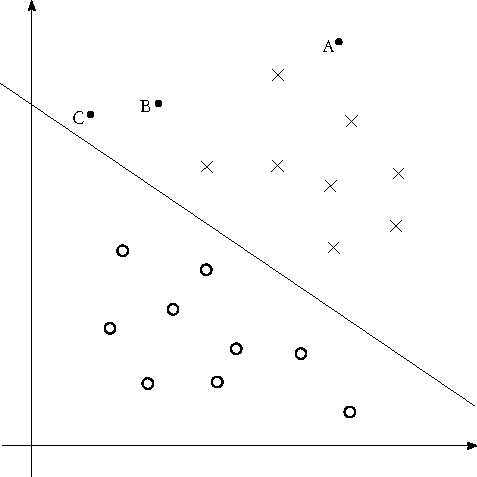
\includegraphics{margin}
  \caption{决策边界}
  \label{fig:margin}
\end{figure}

从图中可以看到A点离决策边界非常远,如果我们在A点处对$y$的值进行预测,我们可以得到一个置信度
非常高的结果$y = 1$。相反,C点离决策边界非常近,虽然我们根据它在决策边界右侧可以预测得到
$y = 1$,但是即便是决策边界的一个微小的变化都会轻易地导致预测结果变为$y = 0$。也就是说A点
处的预测结果比C点处的预测结果具有更高的置信度,而B点处于这两种情况之间。一般来讲,如果一个点
离分类超平面越远,我们的预测结果的置信度就越高。在给定一个训练集的情况下,我们希望找到一个
决策边界能够对训练集中的所有样本都能做出正确并且置信度高的预测。之后我们会用几何间隔的概念
来正式表述这种思想。

\subsubsection{符号定义}

为了表述方便,我们首先需要引入一种新的记法来讨论分类问题。重新明确一下要解决的问题:特征为
$x$,标签为$y$的二分类问题,求一个线性分类器。从现在开始,我们使用$y \in \{-1, 1\}$(而不是
$\{0, 1\}$)来表示类别标签。另外,我们用参数$w, b$(而不是$\theta$)来表示我们的线性分类器,
如式~\ref{equ:chap2:classifier}所示。
\begin{equation}
  \label{equ:chap2:classifier}
  h_{w,b}(x) = g(w^Tx+b)
\end{equation}

此处如果$z \geq 0$那么$g(z) = 1$,否则$g(z) = -1$。

\subsubsection{函数间隔和几何间隔}

下面正式给出函数间隔和几何间隔的定义。给定一个训练样本$(x^{(i)},y^{(i)})$,定义$(w,b)$相对
于训练样本的函数间隔如式~\ref{equ:chap2:fmargin_i}所示。
\begin{equation}
  \label{equ:chap2:fmargin_i}
  \hat{\gamma}^{(i)} = y^{(i)}(w^Tx+b)
\end{equation}

从~\ref{equ:chap2:fmargin_i}式可以看出,在$y^{(i)} = 1$时,为了使函数间隔尽量大(即预测结果
置信度尽量高),我们需要使$w^Tx+b$为一个尽可能大的正数。相反,在$y^{(i)} = -1$时,为了
使函数间隔尽量大,$w^Tx+b$需要为一个尽可能小的负数。此外,$y^{(i)}(w^Tx+b) > 0$意味着我们的
预测结果是正确的。因此,大的函数间隔代表了准确且高置信度的预测结果。

给定一个训练集$S = \{(x^{(i)},y^{(i)});i = 1, ..., m\}$,定义$(w,b)$关于$S$的函数边界为
所有训练样本的函数边界的最小值,记为$\hat{\gamma}$,可以用式~\ref{equ:chap2:fmargin}表示。
\begin{equation}
  \label{equ:chap2:fmargin}
  \hat{\gamma} = \min_{i=1,...,m}\hat{\gamma}^{(i)}
\end{equation}

对于这样一个线性分类器,如果用$2w$和$2b$分别替换$w$和$b$,那么$g(w^Tx+b)=g(2w^Tx+2b)$,$h_{w,b}(x)$
将保持不变。也就是说$g$和$h_{w,b}(x)$仅仅取决于$w^Tx+b$的符号而不是大小。然而将$(w,b)$替换为
$(2w,2b)$会导致函数间隔变为原来的两倍。因此,我们需要引入一些归一化条件,比如令$\|w\|=1$。

下面,我们讨论几何边界。考虑图~\ref{fig:margin2}所示的分类问题:
\begin{figure}[ht] % use float package if you want it here
  \centering
  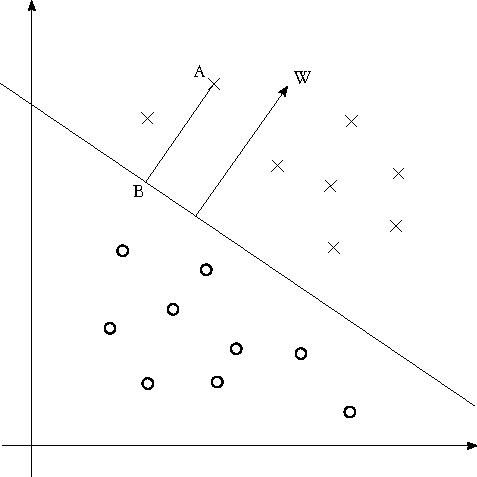
\includegraphics{margin2}
  \caption{几何间隔}
  \label{fig:margin2}
\end{figure}

图中画出了与$(w,b)$所对应的决策边界,以及向量$w$。显然,$w$是垂直于分类超平面的。A点是某个
训练样本的输入$x^{(i)}$,其标签为$y^{(i)} = 1$,到决策边界的距离$\gamma^{(i)}$由线段AB给出。

下面来计算$\gamma^{(i)}$的值。由于$w/\|w\|$是一个与$w$同方向的单位向量,并且A点坐标为$x^{(i)}$,
因此我们可以得到B点的坐标为$x^{(i)} - \gamma^{(i)} \cdot w/\|w\|$。进一步由于B点在决策边界上,
而所有决策边界上的点$x$均满足$w^Tx+b=0$,因此得到:
\begin{equation}
  \label{equ:chap2:gmargin_i_1}
  w^T\left(x^{(i)} - \gamma^{(i)}\frac{w}{\|w\|}\right) + b = 0
\end{equation}

解得:
\begin{equation}
  \label{equ:chap2:gmargin_i_2}
  \gamma^{(i)} = \frac{w^Tx^{(i)}+b}{\|w\|} = \left(\frac{w}{\|w\|}\right)^Tx^{(i)} + \frac{b}{\|w\|}
\end{equation}

式~\ref{equ:chap2:gmargin_i_2}对任意正样本(即$y^{(i)} = 1$)成立。对于一般情况,
定义$(w,b)$关于训练样本$(x^{(i)}, y^{(i)})$的几何间隔为:
\begin{equation}
  \label{equ:chap2:gmargin_i_3}
  \gamma^{(i)} = y^{(i)}\left(\left(\frac{w}{\|w\|}\right)^Tx^{(i)} + \frac{b}{\|w\|}\right)
\end{equation}

从~\ref{equ:chap2:gmargin_i_3}式可以看出,如果$\|w\|=1$,那么函数间隔将等于几何间隔。可以看出
与函数间隔不同的是如果我们用$2w$和$2b$分别替换$w$和$b$,那么几何间隔将不会发生改变。也正是由于
几何间隔相对于参数缩放的这种不变性,当我们使用训练数据来拟合$w$和$b$的时候,我们可以引入任意
的缩放约束,而不会改变模型本身。比如,可以令$\|w\|=1$,或者$|w_1|=5$,或者$|w_1+b|+|w_2|=2$等。

同样,给定一个训练集$S=\{(x^{(i)},y^{(i)});i=1,...,m\}$,定义$(w,b)$关于$S$的几何间隔
为所有训练样本的几何间隔的最小值,如~\ref{equ:chap2:gmargin}式所示。
\begin{equation}
  \label{equ:chap2:gmargin}
  \gamma=\min_{i=1,...,m}\gamma^{(i)}
\end{equation}

\subsubsection{最优间隔分类器}

给定一个训练集,从前面的讨论可以得到一个自然的结论:通过寻找最大化几何间隔的决策边界,就能得到
一个在训练集上拟合得很好的分类器。假设训练集上的两类样本是线性可分的,即存在分类超平面可以完全
将两类样本分开,那么寻找最大化几何间隔的超平面的问题可以表述为~\ref{equ:chap2:opt1}式所示的优化
问题。
\begin{equation}
  \label{equ:chap2:opt1}
  \begin{aligned}
    \max_{\gamma,w,b} &
    & & \gamma \\
    \text{s.t.} &
    & & y^{(i)}\left(w^Tx^{(i)}+b\right)\geq \gamma, i=1,...,m \\
    \quad &
    & & \|w\|=1
  \end{aligned}
\end{equation}

即最大化$\gamma$,使得每个训练样本的函数间隔都至少是$\gamma$。约束条件$\|w\|=1$保证了函数间隔和
几何间隔相等,从而保证了所有训练样本的几何间隔也至少是$\gamma$。

由于约束条件$\|w\|=1$是非凸的,因此这个问题不易直接用标准优化软件工具求解。因此将其转化为
~\ref{equ:chap2:opt2}式所示的优化问题。
\begin{equation}
  \label{equ:chap2:opt2}
  \begin{aligned}
    \max_{\hat{\gamma},w,b} &
    & & \frac{\hat{\gamma}}{\|w\|} \\
    \text{s.t.} &
    & & y^{(i)}\left(w^Tx^{(i)}+b\right)\geq \hat{\gamma}, i=1,...,m
  \end{aligned}
\end{equation}

由于几何间隔和函数间隔之间存在关系$\gamma=\hat{\gamma}/\|w\|$,因此我们最大化$\hat{\gamma}/\|w\|$,
使得所有训练样本的函数间隔至少为$\hat{\gamma}$。这样虽然去掉了约束条件$\|w\|=1$,但是引入了非凸
的目标函数$\frac{\hat{\gamma}}{\|w\|}$。

前面提到我们可以在$w$和$b$上增加任意一个缩放约束条件而不改变问题本身。因此我们可以令$w,b$关于训练集
的函数间隔等于1。
\begin{equation}
  \label{equ:chap2:constrain}
  \hat{\gamma} = 1
\end{equation}

将~\ref{equ:chap2:constrain}式代入~\ref{equ:chap2:opt2},并将最大化$\hat{\gamma}/\|w\|=1/\|w\|$
替换为最小化$\frac{1}{2}\|w\|^2$,可以得到~\ref{equ:chap2:opt3}式所示的优化问题。
\begin{equation}
  \label{equ:chap2:opt3}
  \begin{aligned}
    \min{w,b} &
    & & \frac{1}{2}\|w\|^2 \\
    \text{s.t.} &
    & & y^{(i)}\left(w^Tx^{(i)}+b\right)\geq 1, i=1,...,m
  \end{aligned}
\end{equation}

\subsubsection{拉格朗日对偶问题}

虽然~\ref{equ:chap2:opt3}式表示的优化问题可以使用商业的二次规划(Quadratic Programming, QP)
代码来求解,但是一般情况下我们都是选择将其转化为拉格朗日对偶形式来求解。这对我们使用核函数来
使模型更好地应用于高维特征空间是至关重要的。另外,其对偶形式可以通过一些迭代算法来求解,
通常情况下比直接使用QP软件求解更加高效。

~\ref{equ:chap2:opt3}式表示的原问题对应的拉格朗日函数如~\ref{equ:chap2:lagrangian}式所示。
\begin{equation}
  \label{equ:chap2:lagrangian}
  \mathcal{L}(w,b,\alpha)=\frac{1}{2}\|w\|^2-\sum_{i=1}^m \alpha_i\left[y^{(i)}\left(w^Tx^{(i)}+b\right)-1\right]
\end{equation}

固定$\alpha$,最小化$\mathcal{L}(w,b,\alpha)$,即$\mathcal{L}$关于$w$和$b$的偏导数为0:
\begin{equation}
  \label{equ:chap2:derivative_w}
  \nabla_w\mathcal{L}(w,b,\alpha)=w-\sum_{i=1}^{m}\alpha_iy^{(i)}x^{(i)}=0
\end{equation}

解得:
\begin{equation}
  \label{equ:chap2:expression_w}
  w=\sum_{i=1}^{m}\alpha_iy^{(i)}x^{(i)}
\end{equation}

$\mathcal{L}$关于$b$的偏导数为0,得到:
\begin{equation}
  \label{equ:chap2:derivative_b}
  \frac{\partial}{\partial b}\mathcal{L}(w,b,\alpha)=\sum_{i=1}^m\alpha_iy^{(i)}=0
\end{equation}

将~\ref{equ:chap2:expression_w}式和~\ref{equ:chap2:derivative_b}式代入~\ref{equ:chap2:lagrangian}式
化简可得:
\begin{equation}
  \label{equ:chap2:dual_objective}
  \mathcal{L}(w,b,\alpha)=\sum_{i=1}^m\alpha_i-\frac{1}{2}\sum_{i,j=1}^m
  y^{(i)}y^{(j)}\alpha_i\alpha_j(x^{(i)})^Tx^{(j)}
\end{equation}

加上拉格朗日乘子$\alpha_i$非负的约束条件,以及~\ref{equ:chap2:derivative_b}式的约束条件,可以得到
对偶优化问题如~\ref{equ:chap2:dual_opt}式所示。
\begin{equation}
  \label{equ:chap2:dual_opt}
  \begin{aligned}
    \max_{\alpha} &
    & & \sum_{i=1}^m\alpha_i-\frac{1}{2}\sum_{i,j=1}^m
    y^{(i)}y^{(j)}\alpha_i\alpha_j\langle x^{(i)},x^{(j)}\rangle\\
    \text{s.t.} &
    & & \alpha_i\geq 0, i=1,...,m \\
    \quad &
    & & \sum_{i=1}^m\alpha_iy^{(i)}=0
  \end{aligned}
\end{equation}

针对这个优化问题,已经有很多基于迭代的算法被设计出来,其中最经典的是序贯最小优化算法
(SMO, Sequential Minimal Optimization)~\cite{platt1998sequential},
很多其他算法都是基于该算法设计的。这些算法使得我们不必直接通过二次规划的方式求解该优化问题,
保证了模型在特征维度很大或者样本数量很多的情况下仍然能够有效求解。

当我们获得对偶问题的最优解$\alpha^*$之后,可以通过~\ref{equ:chap2:expression_w}式来计算$w^*$,
并通过~\ref{equ:chap2:expression_b}式来计算$b^*$。
\begin{equation}
  \label{equ:chap2:expression_b}
  b^*=-\frac{\max_{i:y^{(i)}=-1}{w^*}^Tx^{(i)}+\min_{i:y^{(i)}=1}{w^*}^Tx^{(i)}}{2}
\end{equation}

最后,我们可以通过计算${w^*}^Tx+b^*$的值来对样本$x$的标签进行预测,如果该值大于0,那么将预测$y=1$,
反之则预测$y=-1$。

\subsubsection{不可分的情况及正则化}

我们在前面推导SVM模型的时候都假定数据是线性可分的,但是并不能保证事实情况总是如此。
此外,即便是能够找到这样一个分类超平面, 也不一定是就是我们想要的结果,
因为这样的分类超平面可能是受到了一些异常点的干扰。举个例子,
图~\ref{fig:margin3}显示了一个最优分类超平面,当一个异常点被加入到左上角区域时
(如~\ref{fig:margin4}所示),分类超平面产生一个非常大的变动,导致分类器的间隔急剧减小。
\begin{figure}[ht]
  \centering%
  \subcaptionbox{正常情况下的决策面\label{fig:margin3}} %标题的长度,超过则会换行,如下一个小图。
  {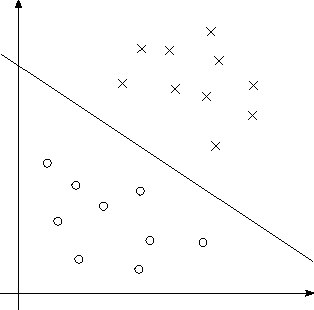
\includegraphics{margin3}}%
  \hspace{6em}%
  \subcaptionbox{有异常点时的决策面\label{fig:margin4}}
  {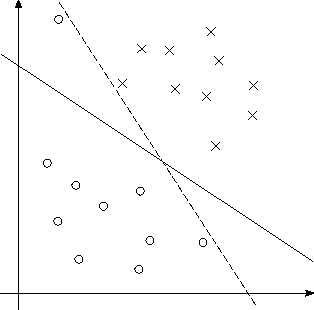
\includegraphics{margin4}}
  \caption{决策面受异常点干扰示例}
  \label{fig:margin3+4}
\end{figure}

为了使得模型在非线性可分的情况下仍然有效,同时对异常点的干扰更加鲁棒,我们将原来的优化问题
重新写为~\ref{equ:chap2:opt_reg}式:
\begin{equation}
  \label{equ:chap2:opt_reg}
  \begin{aligned}
    \min{w,b} &
    & & \frac{1}{2}\|w\|^2+C\sum_{i=1}^m\xi_i \\
    \text{s.t.} &
    & & y^{(i)}\left(w^Tx^{(i)}+b\right)\geq 1-\xi_i, i=1,...,m \\
    \quad &
    & & \xi_i \geq 0, i=1,...,m
  \end{aligned}
\end{equation}

即允许样本的函数间隔小于1(等价于被错分),并且在目标函数中引入一个惩罚项$C\xi_i$。参数C
控制惩罚向所占的权重,被称为惩罚因子。同样地,我们可以得到该优化问题的拉格朗日对偶问题,如
~\ref{equ:chap2:dual_opt_reg}所示。
\begin{equation}
  \label{equ:chap2:dual_opt_reg}
  \begin{aligned}
    \max_{\alpha} &
    & & \sum_{i=1}^m\alpha_i-\frac{1}{2}\sum_{i,j=1}^m
    y^{(i)}y^{(j)}\alpha_i\alpha_j\langle x^{(i)},x^{(j)}\rangle\\
    \text{s.t.} &
    & & 0\leq\alpha_i\leq C, i=1,...,m \\
    \quad &
    & & \sum_{i=1}^m\alpha_iy^{(i)}=0
  \end{aligned}
\end{equation}

\subsubsection{核函数}

从~\ref{equ:chap2:dual_opt_reg}中可以看出,模型可以写成一个完全关于内积$\langle x,z\rangle$的形式,
意味着如果我们使用一种特征映射$\phi$将输入特征$x$变换到空间$\phi(x)$,那么我们可以将所有的内积
替换为$\langle\phi(x),\phi(z)\rangle$。一般地,给定一种特征映射$\phi$,我们定义与之对应的核函数如
~\ref{equ:chap2:kernel}所示。
\begin{equation}
  \label{equ:chap2:kernel}
  K(x,z)=\phi(x)^T\phi(z)
\end{equation}

特别地,当$\phi(x)=x$时,$K(x,z)=\langle x,z\rangle$,我们称之为线性核,此时模型即为
~\ref{equ:chap2:dual_opt_reg}式所示。除此之外,还有很多常用的核函数,举例如下:

1)多项式核函数
\begin{equation}
  \label{equ:chap2:polynomial_kernel}
  K(x,z)=(x^Tz+c)^d
\end{equation}

2)高斯核函数
\begin{equation}
  \label{equ:chap2:gauss_kernel}
  K(x,z)=\exp\left(-\frac{\|x-z\|^2}{2\sigma^2}\right)
\end{equation}

3)sigmoid核函数
\begin{equation}
  \label{equ:chap2:sigmoid_kernel}
  K(x,z)=\tanh(\alpha x^Tz+c)
\end{equation}

\section{基于支持向量机的级联故障诊断模型}

\subsection{基于下采样的单一尺度特征提取方法}

给定一个信号片段$x$,其采样点个数为$N$,即$x=(x_1,x_2,...,x_N)^T$,我们希望得到的特征个数
为$L$。首先我们对$x$进行~\ref{equ:chap2:rdft}式所示的实数形式的离散傅立叶变换,得到RDFT
频谱序列$\hat{X}$,由~\ref{subsection:rdft}节中的介绍可知,$\hat{X}$的维度也是$N$,即
$\hat{X} = (\hat{X}_1, \hat{X}_2, ..., \hat{X}_N)^T$。为了避免样本间相位不同对最终模型的
诊断精度产生影响,同时也为了避免在后续的操作中正负值之间相互抵消,我们对RDFT频谱序列取了
绝对值,即$X = (|\hat{X}_1|, |\hat{X}_2|, ..., |\hat{X}_N|)^T$,本文中之后提到的频谱序列
均是指$X$。接着我们使用平均值下采样来进一步提取特征,将序列$X$等分为$L$个连续
的小区间,并且对各个区间内的值进行平均,得到长度为L的特征向量$V=(V_1,V_2,...,V_L)^T$。
这个过程可以用~\ref{equ:chap2:pooling}式表示,其中$[N/L]$表示不大于$N/L$的最大整数。
\begin{equation}
  \label{equ:chap2:pooling}
  V_k=\frac{1}{[N/L]}\sum_{j=1}^{[N/L]}X_{(k-1)[N/L]+j}, k=1,2,...,L
\end{equation}

使用这样一种特征提取过程的优势在于,相对于直接使用信号频谱序列作为输入特征,
我们可以在保证其整体分布趋势近似不变的同时,大幅度地降低特征向量的维度,
从而提升分类器训练和预测过程的速度,保证诊断过程的是实时性。此外,在特征提取阶段
使用平均值下采样还可以降低某些特定频段的噪声所带来的影响,使得整个模型具有更好的
鲁棒性。此外,我们在使用平均值下采样的过程中,设定了一个参数$L$,也就是最终得到的
特征个数,我们会在之后的仿真实验中对比该参数的变化对模型的影响,从而选择最佳的参数值。

图~\ref{fig:average_pooling}显示了一个采样点数为384的信号片段,其对应的频谱序列,
以及使用平均值下采样提取的特征个数为32的特征向量。
\begin{figure}[ht] % use float package if you want it here
  \centering
  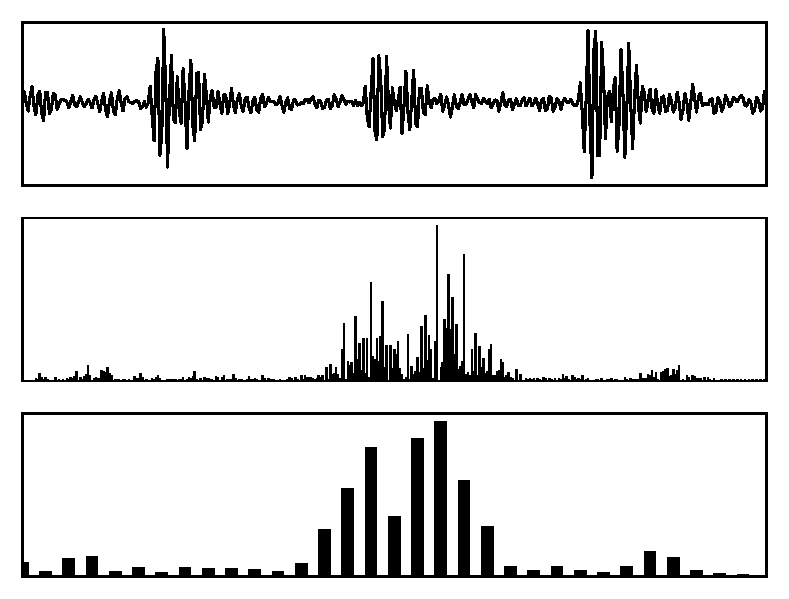
\includegraphics[height=8cm]{average_pooling}
  \caption{原始信号片段,RDFT频谱和特征向量}
  \label{fig:average_pooling}
\end{figure}

\subsection{分类模型}
\label{subsection:cascade_model}

虽然我们可以将提取到的特征向量直接输入到一个多分类模型中进行训练,就可以完成故障分类
的任务,但是在某些特定的情况下,尤其是当数据的类别标签具有明显的层次性(比如在故障诊断
问题当中,最常见的就是存在多种不同的故障位置,并且每一类故障位置可能会进一步有不同的
故障尺寸等等)的时候,设计一个由多个子分类器构成的级联分类器往往会更加有效。

假设在一个故障诊断问题中,存在三类可能的故障位置,我们记为位置A、位置B、位置C,
每一类故障位置都可能会发生3种不同程度的故障,我们记为尺寸1、尺寸2、尺寸3,同时还有一类
是正常样本。那么我们可以针对故障类别的这种层次性,设计一个由5个自分类器构成的级联分类
过程,如图~\ref{fig:cascade_classifier}所示。
\begin{figure}[ht] % use float package if you want it here
  \centering
  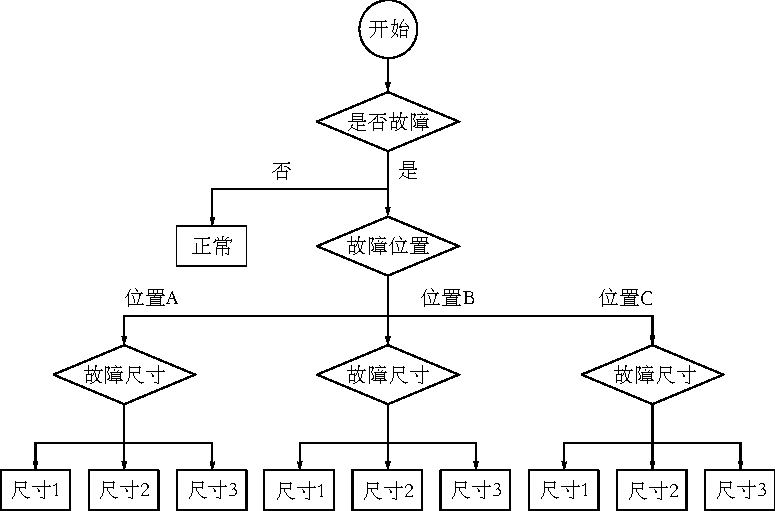
\includegraphics[height=9cm]{cascade_classifier}
  \caption{级联分类过程示意图}
  \label{fig:cascade_classifier}
\end{figure}

图中每个菱形表示一个子分类器,可以根据实际情况采用不同的算法实现,不同子分类器所用的
算法也不一定相同。图中的每一个矩形框代表一种故障类型,可以看出这个例子中总共有10类样本,
其中一类是正常样本。可以看出,整个级联分类过程整体上分为三个阶段,第一个阶段由一个子分
类器判断是否为故障样本;接下来一个阶段有一个子分类器判断故障发生的位置;最后一个阶段
用三个子分类器分别判断故障的尺寸。

\section{实验仿真}

\subsection{实验数据}

本文的所有仿真实验所用的数据均是来自凯斯西储大学(Case Western Reserve University, CWRU)
的滚动轴承加速度测量数据,其中包括正常工作下的轴承数据和在各种不同故障位置和故障
尺寸下的轴承数据。在旋转机械故障诊断领域,该数据集已经成为标准的测试数据集之一,已经有很多
研究人员使用该数据集来仿真测试其故障诊断模型。

数据采集的实验装置如图~\ref{fig:teststand}所示,测试台由一个2马力的三相感应电机(左)、
扭矩传感器/编码器(中间)、测力计(右)和控制电子设备(图中未显示)组成。 
用来收集振动数据的加速度传感器被磁性底座固定在轴承上方的机壳上,处于电机外壳的驱动端和
风扇端的12点钟位置。实验中使用16通道DAT记录仪收集振动信号,并在Matlab环境中进行后续处理。
所有数据文件均采用Matlab(*.mat)格式保存。该数据集以12kHz的采样频率收集和记录数据,另外
也采集了采样频率为48kHz时的数据,用于驱动端的轴承故障研究。
\begin{figure}[ht] % use float package if you want it here
  \centering
  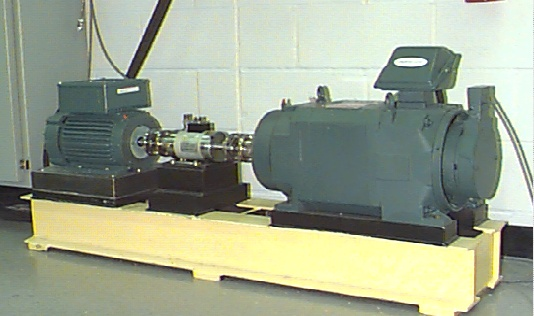
\includegraphics[height=6cm]{teststand}
  \caption{级联分类过程示意图}
  \label{fig:teststand}
\end{figure}

数据采集的实验过程中所用的轴承包括两种,一种是型号为6205-2RS JEM的SKF深沟型轴承,
另一种是型号为6203-2RS JEM的SKF深沟型轴承,表~\ref{tab:bearing_params}列出了型号为
6205-2RS JEM的SKF深沟型轴承的一些主要的几何参数。
\begin{table}[htb]
  \centering
  \begin{minipage}[t]{0.8\linewidth} % 如果想在表格中使用脚注,minipage是个不错的办法
  \caption{6205-2RS JEM SKF深沟型轴承几何参数}
  \label{tab:bearing_params}
    \begin{tabularx}{\linewidth}{lXXXXX}
      \toprule[1.5pt]
      滚珠个数 & 内圈直径(英寸)& 外圈直径(英寸)& 轴承厚度(英寸)& 滚珠直径(英寸)& 轴承节径(英寸) \\\midrule[1pt]
      9 & 0.9843 & 2.0472 & 0.5906 & 0.3126 & 1.537 \\\bottomrule[1.5pt]
    \end{tabularx}
  \end{minipage}
\end{table}

轴承的状态除了正常之外,还有内圈故障、钢球故障和外圈故障三种类型,使用火花放电
的方法在测试轴承上引入7密耳、14密耳、21密耳、28密耳(1密尔=0.001英尺)四种不同损伤直径的
单点故障。电机的负载可以通过风机来调节,可以产生0-3马力的载荷,从而可以研究不同负载情况下
轴承的故障特征。

为了验证本文在各章节中设计的故障诊断模型对故障位置及故障尺寸的识别能力,本文选取了在采样频率为
12kHz,负载为0马力情况下的12种不同类别的数据,对所设计的模型进行训练和测试。这12类样本对应
的故障位置和故障尺寸如表~\ref{tab:class_desc}所示。
\begin{table}[htb]
  \centering
  \begin{minipage}[t]{0.8\linewidth} % 如果想在表格中使用脚注,minipage是个不错的办法
  \caption{12类数据对应的故障位置和尺寸}
  \label{tab:class_desc}
    \begin{tabularx}{\linewidth}{lXX}
      \toprule[1.5pt]
      类别标签 & 故障位置 & 故障尺寸(英寸) \\\midrule[1pt]
      0 & 无 & 无 \\
      1 & 钢球 & 0.007 \\
      2 & 钢球 & 0.014 \\
      3 & 钢球 & 0.021 \\
      4 & 钢球 & 0.028 \\
      5 & 内圈 & 0.007 \\
      6 & 内圈 & 0.014 \\
      7 & 内圈 & 0.021 \\
      8 & 内圈 & 0.028 \\
      9 & 外圈 & 0.007 \\
      10 & 外圈 & 0.014 \\
      11 & 外圈 & 0.021 \\
      \bottomrule[1.5pt]
    \end{tabularx}
  \end{minipage}
\end{table}

\subsection{实验过程}

从表~\ref{tab:class_desc}中可以看到,除了一类正常数据,以及在故障尺寸为0.028英尺时包含钢球和内圈两种故障位置,
其余的三类故障尺寸都分别包含钢球、内圈和外圈三种故障位置,一共是12类数据。根据
~\ref{subsection:cascade_model}节中的级联分类思路,以及本文所使用的数据的特点,我们设计了
如图~\ref{fig:cascade_classifier_exp}所示的级联故障诊断模型,分类器输出的类别标签与实际样本的对应关系
参见表~\ref{tab:class_desc}。
\begin{figure}[ht] % use float package if you want it here
  \centering
  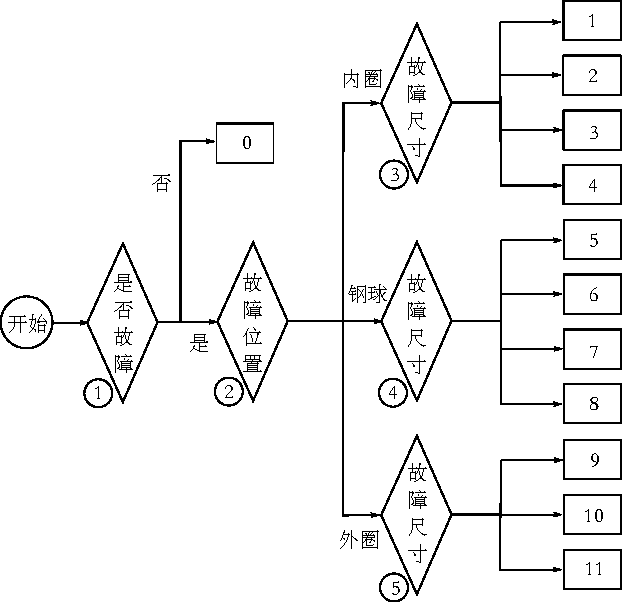
\includegraphics[height=11cm]{cascade_classifier_exp}
  \caption{CWRU数据级联分类模型}
  \label{fig:cascade_classifier_exp}
\end{figure}

在这个级联故障诊断模型中,我们总共有5个子分类器,每个子分类器我们使用了支持向量机算法,
并且个分类器之间单独进行训练,最后在预测阶段按照图~\ref{fig:cascade_classifier_exp}中
显示的级联过程逐步进行预测,得到最终的预测标签。图中各分类器的功能描述如
表~\ref{tab:classifier_desc}所示,其中12类数据的标签对应的故障情况参见表~\ref{tab:bearing_params}。
\begin{table}[htb]
  \centering
  \begin{minipage}[t]{0.8\linewidth} % 如果想在表格中使用脚注,minipage是个不错的办法
  \caption{各子分类器详细说明}
  \label{tab:classifier_desc}
    \begin{tabularx}{\linewidth}{lXXX}
      \toprule[1.5pt]
      分类器序号 & 输出标签个数 & 训练所用数据标签 & 分类器功能 \\\midrule[1pt]
      1 & 2 & 0-11 & 判断样本是否故障\\
      2 & 3 & 1-11 & 判断故障样本的故障位置\\
      3 & 4 & 1-4 & 判断钢球故障样本的故障尺寸\\
      4 & 4 & 5-8 & 判断内圈故障样本的故障尺寸\\
      5 & 3 & 9-11 & 判断外圈故障样本的故障尺寸\\
      \bottomrule[1.5pt]
    \end{tabularx}
  \end{minipage}
\end{table}

由于CWRU数据集中每一种类别的数据都存储在一个Matlab文件(*.mat)中,并且每一个文件中都
包含了一段至少12000个连续的采样点。因此,为了获得足够数量的样本对设计的故障诊断模型
进行训练和预测,我们从每个数据文件中随机地截取M个长度为N的信号片段,并且将其中的3/4M个
信号片段作为训练样本,其余M/4个信号片段作为预测样本。在选择N值的时候,一方面要保证能够
从有限的采样点中截取到足够多的信号片段来训练我们的模型,因此N值不能太大;另一方面要保证
截取的长度为N的信号片段中能够包含足够的信息,因此N值也不能太小。在本文的所有仿真实验中
均使用$N=384$。

\subsection{实验结果及分析}
\label{subsection:cascade_result}

图~\ref{fig:series}是从表~\ref{tab:class_desc}中所列的12类数据中随机截取的信号片段的
原始波形,图中从左至右,从上到下依次对应类别标签为0-11的样本。每一类数据我们都随机地
显示了3信号样本。
\begin{figure}[ht] % use float package if you want it here
  \centering
  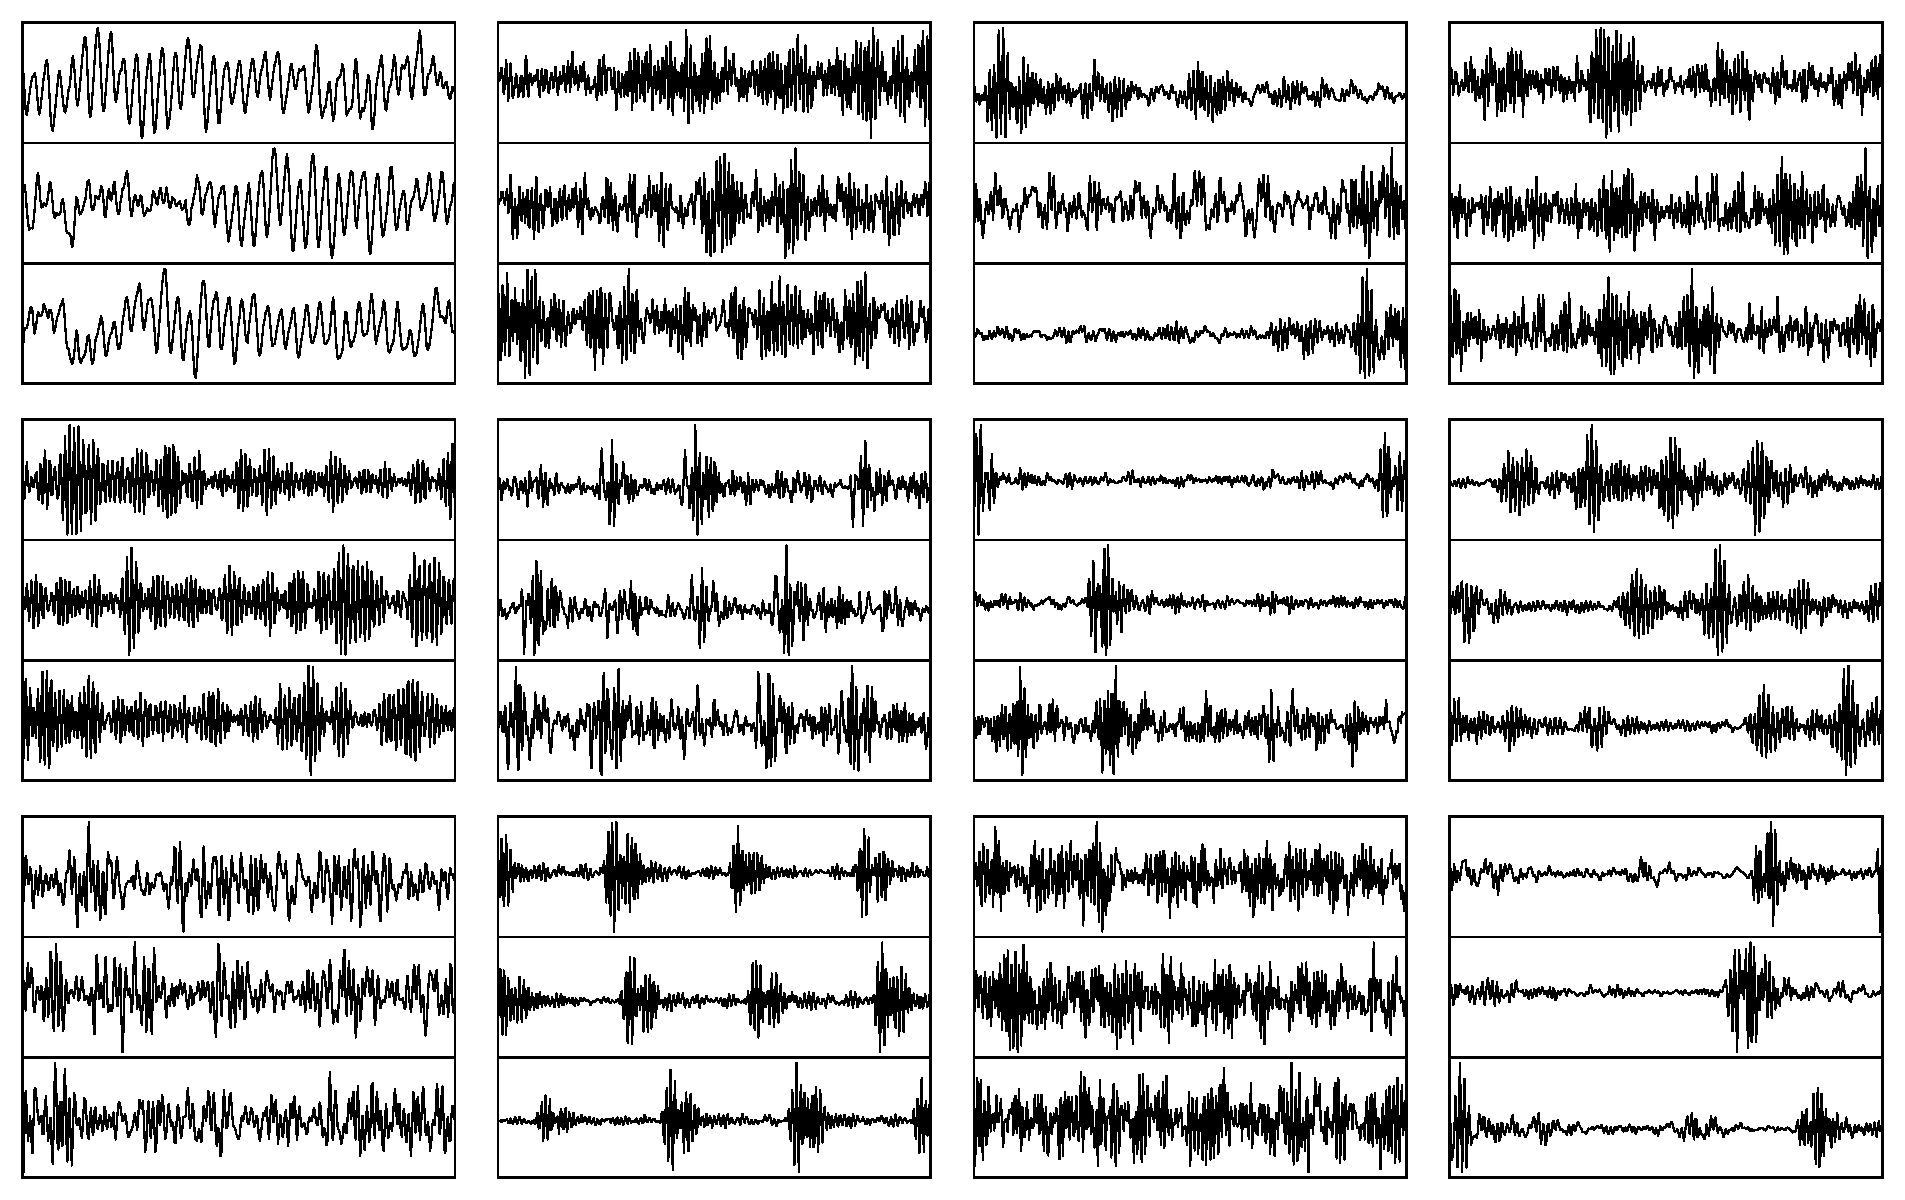
\includegraphics[height=9cm]{series}
  \caption{各类信号片段原始波形}
  \label{fig:series}
\end{figure}

从图中可以看出,由于样本的截取过程是随即进行的,因此同一类样本间存在很大的相位差别,
因此如果直接使用原始信号片段来训练分类器的效果比较差。使用本章中基于下采样的特征提取方法,
对图~\ref{fig:series}中列出的12个信号频段进行特征提取,所获得的特征向量如图
~\ref{fig:average_pooling_features_12}所示。
\begin{figure}[ht] % use float package if you want it here
  \centering
  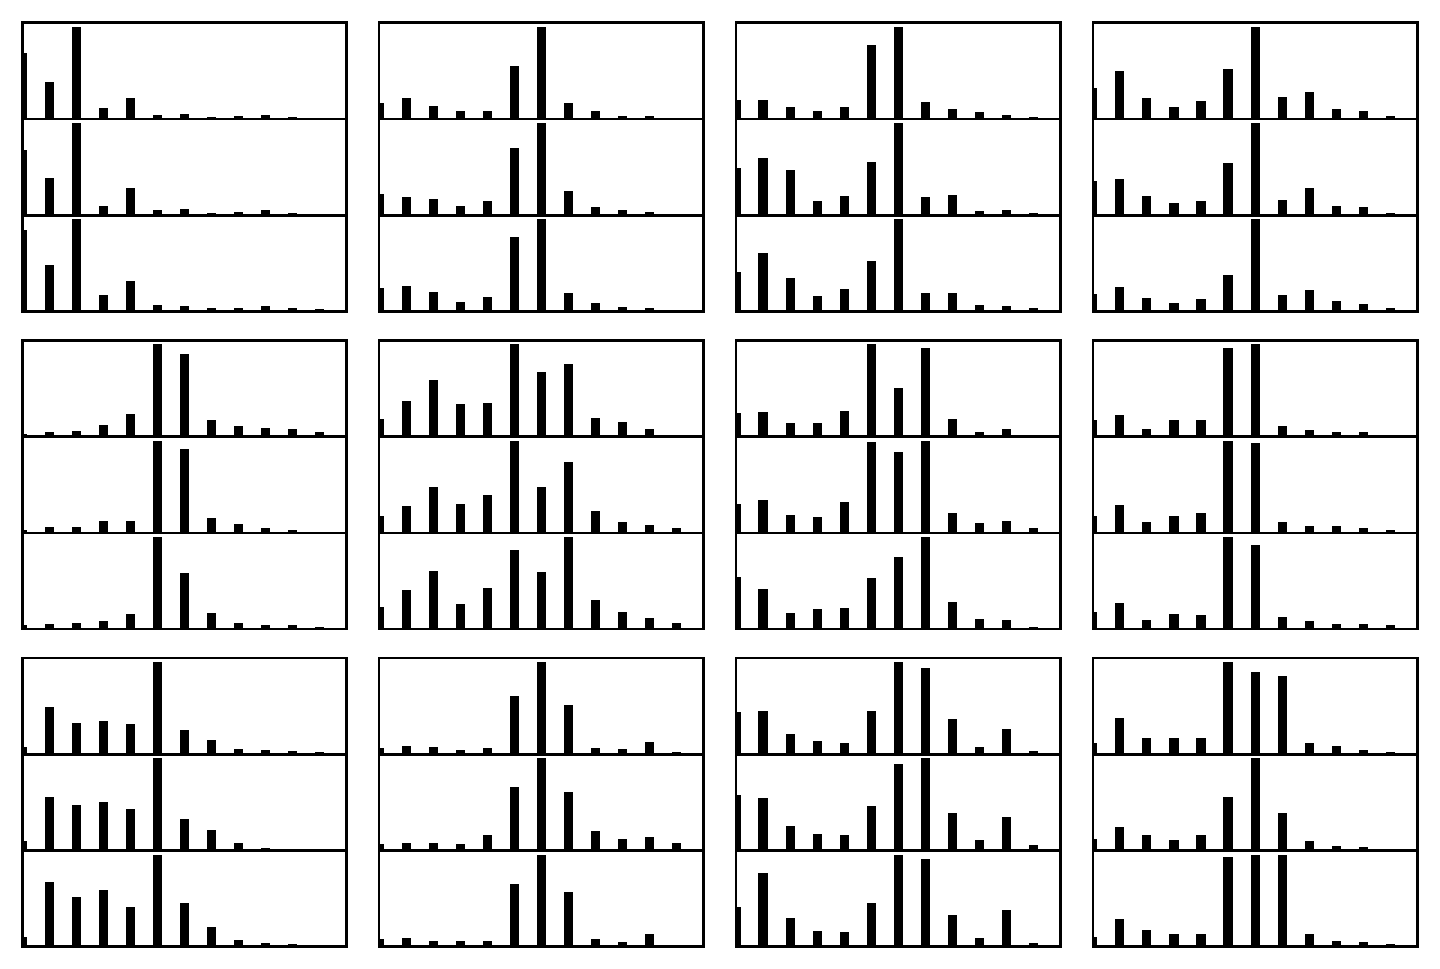
\includegraphics[height=9cm]{average_pooling_features_12}
  \caption{基于RDFT和平均值下采样提取的特征向量}
  \label{fig:average_pooling_features_12}
\end{figure}

可以看出,与图~\ref{fig:series}中显示的原始信号片段相比,使用本章中的特征提取方法获得
的结果作为特征向量时,避免信号片段间相位的差异带来的分类难度,使得类别之间具有更好的区分性,
而同一类样本之间的相似程度也更高,因此能够提升最终的故障诊断精度。另一方面,图
~\ref{fig:average_pooling_features_12}中的特征向量的维度为12,相比于原始信号片段的维度384,
极大程度地降低了特征的维度,加快了模型的训练过程。

此外,本章中设计的特征提取算法中的参数L,也就是最终得到的特征向量的维度,是可以人为指定的,
例如图~\ref{fig:average_pooling_features_12}中显示的是$L=12$时提取的特征向量,当$L=384$时,
相当于直接将信号片段的频谱用作特征向量,如~\ref{fig:average_pooling_features_384}所示。
\begin{figure}[ht] % use float package if you want it here
  \centering
  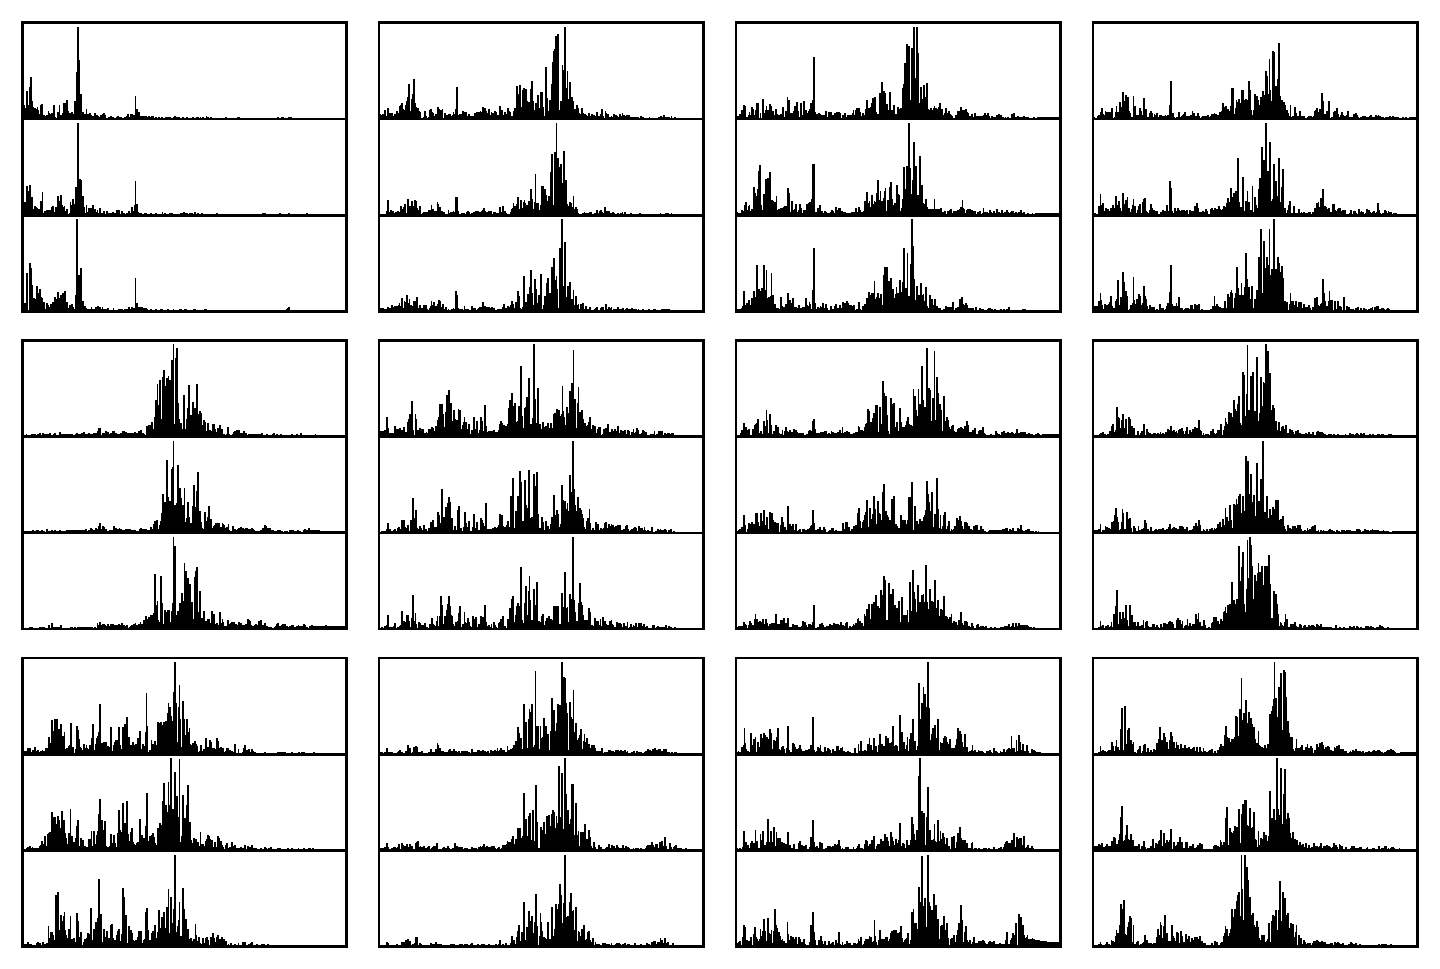
\includegraphics[height=9cm]{average_pooling_features_384}
  \caption{维度为384的特征向量}
  \label{fig:average_pooling_features_384}
\end{figure}

选择适当的特征维度L也是影响模型精度的一个关键因素。如果L值过大,那么下采样在特征提取过程中
起到的作用就相对比较微弱,无法过滤掉信号种特定频段的一些噪声,同时过大的特征维度也会减慢
分类器的训练和预测速度;相反,如果L值过小,那么最终提取的特征向量将会丢失原始信号片段中的
过多信息,因此将会降低分类器的预测精度。因此,我们会从最终训练得到的分类器的预测精度和训练
过程所用时长两方面考虑,来最终选择合适的L值。

分别取特征个数L为3、6、12、24、48、96、192的情况下训练并测试级联分类模型中的5个子分类器,
子分类器使用的是支持向量机算法,核函数使用高斯核函数,算法的参数取值为惩罚因子$C=1$,
高斯核宽度参数$\sigma=L$。整个级联分类模型的预测精度和训练时间如表~\ref{tab:chap2_acc_time}
所示。
\begin{table}[htb]
  \centering
  \begin{minipage}[t]{0.8\linewidth} % 如果想在表格中使用脚注,minipage是个不错的办法
  \caption{不同特征个数下模型的预测精度和训练时间}
  \label{tab:chap2_acc_time}
    \begin{tabularx}{\linewidth}{lXX}
      \toprule[1.5pt]
      特征个数 & 模型预测精度 & 模型训练时间 \\\midrule[1pt]
      3   &  0.6932 & 2.23  \\
      6   &  0.7947 & 0.89  \\
      12  &  0.8784 & 1.03  \\
      24  &  0.9171 & 1.37  \\
      48  &  0.9381 & 2.01  \\
      96  &  0.9297 & 3.22  \\
      192 &  0.9349 & 5.89  \\
      384 &  0.9184 & 11.29 \\
      \bottomrule[1.5pt]
    \end{tabularx}
  \end{minipage}
\end{table}

模型的预测精度和模型训练所用时间随特征个数L的变化趋势如图~\ref{fig:chap2_accs}和
图~\ref{fig:chap2_times}所示。
\begin{figure}[ht] % use float package if you want it here
  \centering
  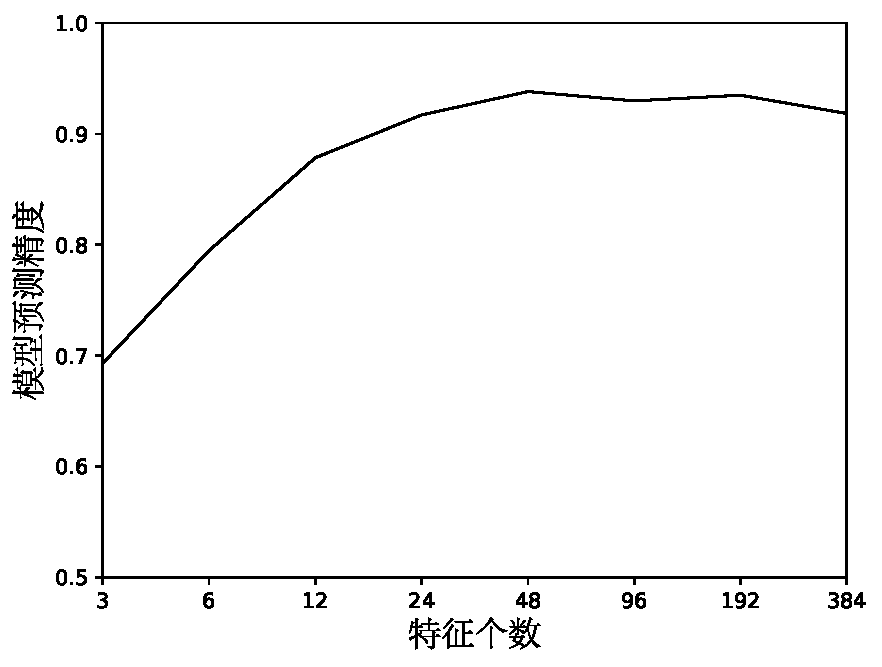
\includegraphics[height=6cm]{chap2_accs}
  \caption{模型预测精度随特征个数的变化情况}
  \label{fig:chap2_accs}
\end{figure}

\begin{figure}[ht] % use float package if you want it here
  \centering
  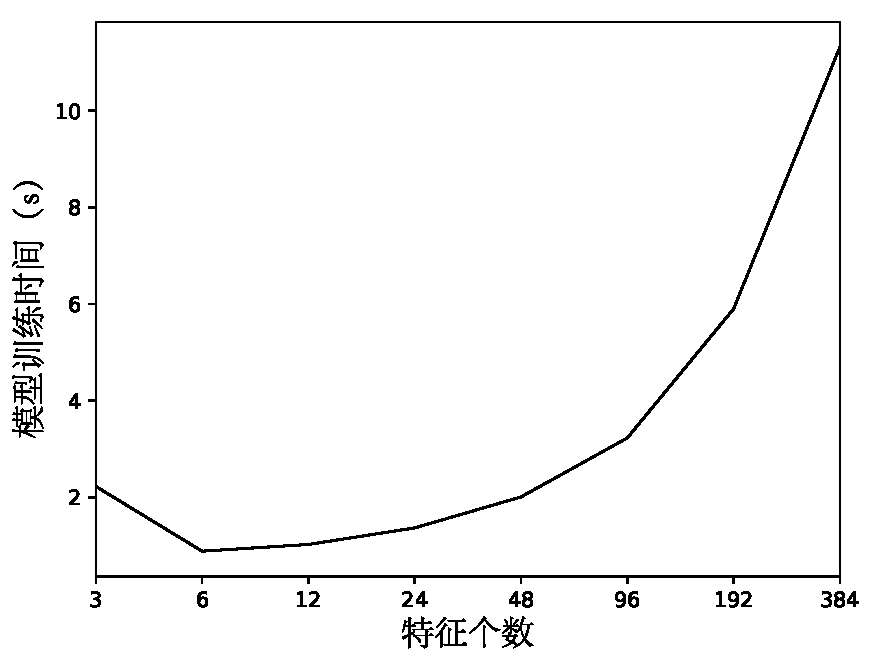
\includegraphics[height=6cm]{chap2_times}
  \caption{模型训练时间随特征个数的变化情况}
  \label{fig:chap2_times}
\end{figure}

从图~\ref{fig:chap2_accs}和图~\ref{fig:chap2_times}可以看出,模型在特征个数取48时,
模型的预测精度达到最高,为93.81\%,并且训练所需时间也相对比较少。因此可以将$L=48$
作为最终的选择。此时模型在测试集上的混淆矩阵如表\ref{tab:chap2:confusion_matrix}所示。
\begin{table}[htb]
  \centering
  \begin{minipage}[t]{0.9\linewidth} % 如果想在表格中使用脚注,minipage是个不错的办法
  \caption{L=48时模型在测试集上的混淆矩阵}
  \label{tab:chap2:confusion_matrix}
    \begin{tabularx}{\linewidth}{l|XXXXXXXXXXXX}
      \toprule[1.5pt]
         &    0 &   1 &   2 &   3 &   4 &   5 &   6 &   7 &   8 &   9 &  10 &  11 \\\midrule[1pt]
      0  & 1579 &   0 &   0 &   0 &   0 &   0 &   0 &   0 &   0 &   0 &   0 &   0 \\
      1  &    0 & 697 &   2 &  11 &   0 &   0 &   0 &   0 &   0 &   0 &   0 &   0 \\
      2  &    0 &  83 & 682 &  18 &   0 &   0 &   0 &   0 &   0 &   0 &   0 &   1 \\
      3  &    0 &  20 &   0 & 765 &   0 &   0 &   0 &   0 &   0 &   0 &   0 &   0 \\
      4  &    0 &   0 &   0 &   0 & 777 &   0 &   0 &   0 &   0 &   0 &   0 &   0 \\
      5  &    0 &   0 &   0 &   0 &   0 & 780 &   0 &   0 &   0 &   0 &   0 &   0 \\
      6  &    0 &   0 &   0 &   0 &   0 &   0 & 784 &   0 &   0 &   0 &   0 &   0 \\
      7  &    0 &   0 &   0 &   0 &   0 &   0 &   0 & 786 &   0 &   0 &   0 &   0 \\
      8  &    0 &   0 &   0 &   0 &   0 &   0 &   0 &   0 & 777 &   0 &   0 &   0 \\
      9  &    0 &   0 &   0 &   0 &   0 &   0 &   0 &   0 &   0 & 785 &   0 &   0 \\
      10 &    0 &   0 &   0 &   0 &   0 &   0 &   0 &   0 &   0 &   0 & 784 &   0 \\
      11 &    0 &   0 &   0 &   0 & 395 &   0 &   1 &   2 &   0 &  93 &   0 & 297 \\
      \bottomrule[1.5pt]
    \end{tabularx}
  \end{minipage}
\end{table}

从混淆矩阵可以看出,类别标签为0、5、8、10的测试样本的预测结果与样本的真实标签
完全一致,其他类别的样本或多或少都存在预测结果错误的情况,尤其是第11类样本(外圈
故障,尺寸为0.021)的样本,在784各样本中有491个样本预测错误。

\section{小结}

本章介绍了信号处理中经常用到的实数形式的傅立叶变换,以及传统的机器学习算法中经典的
支持向量机算法。之后详细介绍了本章中设计的基于单一尺度的故障特征提取方法和基于
支持向量机算法的级联诊断模型。特征提取阶段使用了平均值下采样来对信号片段频谱序列
的特征个数进行压缩,同时也能够减弱信号中特定频谱的噪声对诊断效果的影响。另外,由于我们
通过改变下采样的宽度来控制特征向量的维度,因此我们能够得到不同尺度下的特征,因此我们
通过对比仿真实验考察了不同尺度的特征对诊断模型的影响,最后给出了能够使模型预测精度达到
最高的特征维度。但是我们也分析了该模型在测试集上的预测结果的混淆矩阵,发现在某些类别
的样本上表现并不理想,这也是后面的章节中设计的模型需要进一步提升的地方。

\chapter{单一尺度下基于深度神经网络的故障诊断模型研究}
\label{cha:chapter3}

\section{引言}

在第~\ref{cha:chapter2}章中,我们使用RDFT(实数形式的傅立叶变换)将原始信号片段变换为长度与其
相等的频谱序列,并在此基础上使用平均值下采样的方法进行了特征提取,最后使用所提取的特征训练和
测试一个基于SVM的级联分类模型,达到了不错的预测精度。平均值下采样的过程是将长度为$N$的序列$X$
等分为$L$个连续的小区间,然后在各区间内计算均值,最后将这$L$个均值排成的向量作为结果。通常,
我们将$F=X/L$称为下采样的核宽度。除了平均值下采样之外,最常用的还有最大值下采样,具体的计算过
程本章会详细介绍。第~\ref{cha:chapter2}章的仿真实验中我们也考察了使用不同核宽度的平均值下采样
进行特征提取对模型最终的预测精度的影响,我们发现随着核宽度从$2^0$到$2^7$的变化过程中,模型的
预测精度会呈现出先增高后降低的趋势。下采样实际上是用局部区域的平均或显著值来代替相应区域,从
而降低特征维度的过程。因此合适的下采样核宽度能够起到提取显著特征,缩减特征维度的作用;但是过大
的下采样核宽度会给原始特征造成破坏性,导致信息丢失严重。因此实际应用中最常见的是核宽度$F=2$的
下采样。第~\ref{cha:chapter2}章虽然在下采样核宽度$F=8$也就是$L=48$时能够获得93.81\%的预测精度,
但是分析测试集上预测结果的混淆矩阵可以发现,在个别类别的样本上表现比较差,较大的核宽度可能是
导致这种结果的原因之一。图~\ref{fig:single_pooling}是第~\ref{cha:chapter2}章中用到的单层下采样
提取特征的示意图。
\begin{figure}[ht]
  \centering%
  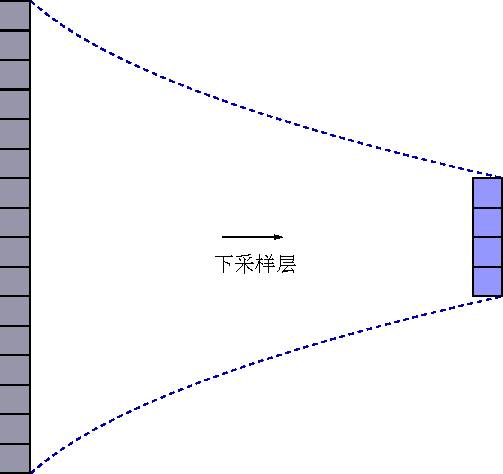
\includegraphics{single_pooling}
  \caption{单个核宽度为4的下采样}
  \label{fig:single_pooling}
\end{figure}

在卷积神经网络(Convolutional Neural Network, CNN)中,通常会有多个核宽度$F=2$的下采样操作,并
且在两个下采样操作之间往往会有至少一个卷积层。图~\ref{fig:multi_pooling}是CNN中多层下采样操作筛
选特征的示意图。使用这样的结构来处理信号频谱序列,不但可以逐层提取或筛选特征,降低特征的维度,
而且可以避免使用单个下采样操作时,核宽度过大所带来的信息丢失。
\begin{figure}[ht]
  \centering%
  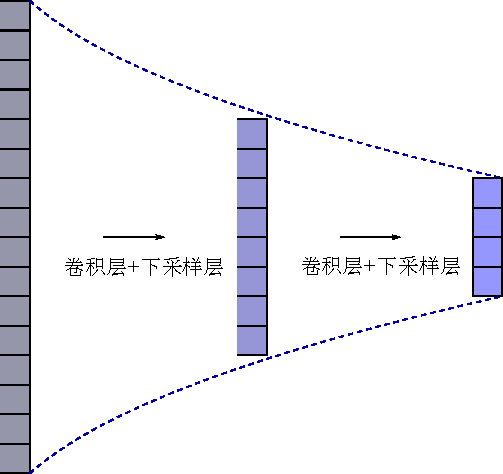
\includegraphics{multi_pooling}
  \caption{两个核宽度为2的下采样}
  \label{fig:multi_pooling}
\end{figure}

本章首先对神经网络相关的概念做了简单介绍,包括神经元的基本构成、一般神经网络的结构以及神经网络
的训练算法——反向传播算法。接下来我们介绍了卷积神经网络的结构、卷积神经网络中常用的三种层:卷积
层、下采样层和全连接层。然后我们详细介绍了本章基于卷积神经网络设计的故障诊断模型,最后在CWRU数
据集上进行仿真实验,并且得到了比第~\ref{cha:chapter2}章更好的预测效果。

\section{基本理论}

\subsection{神经网络}
\label{subsection:nn}

\subsubsection{神经元}

在正式介绍神经网络之前,我们首先需要了解神经网络的基本组成单元——神经元。图~\ref{fig:neuron}是
一个神经元的基本结构。
\begin{figure}[ht]
  \centering%
  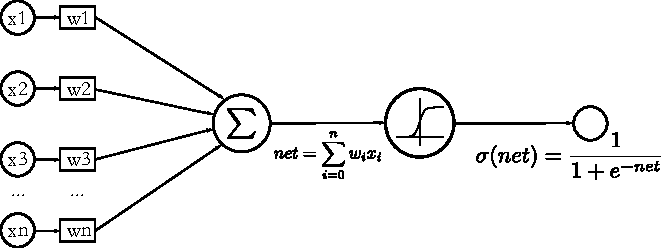
\includegraphics{neuron}
  \caption{神经元结构}
  \label{fig:neuron}
\end{figure}

假设神经元的输入记为向量$x$,相应的权重向量记为$w$,激活函数取sigmoid函数,那么神经元的输出$y$
可以通过~(\ref{equ:chap3:neuron1})式得出:
\begin{equation}
  \label{equ:chap3:neuron1}
  y = \text{sigmoid}(w^Tx)
\end{equation}

sigmoid函数的定义如~(\ref{equ:chap3:neuron2})所示。
\begin{equation}
  \label{equ:chap3:neuron2}
  \text{sigmoid}(x) = \frac{1}{1+e^{-x}}
\end{equation}

将~(\ref{equ:chap3:neuron2})代入~(\ref{equ:chap3:neuron1})可得:
\begin{equation}
  \label{equ:chap3:neuron3}
  y = \frac{1}{1+e^{-w^Tx}}
\end{equation}

sigmoid函数的图像如图~\ref{fig:sigmoid}所示。
\begin{figure}[ht]
  \centering
  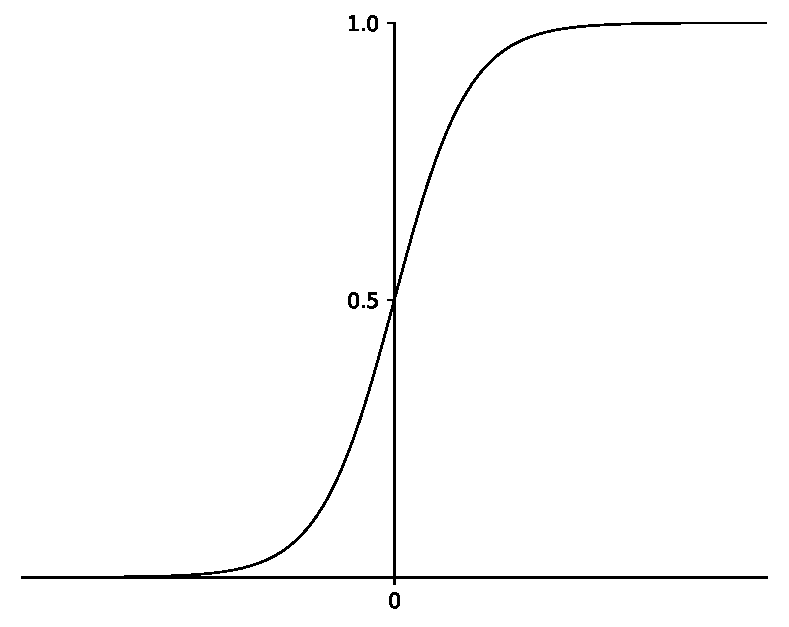
\includegraphics[height=6cm]{sigmoid}
  \caption{sigmoid函数图像}
  \label{fig:sigmoid}
\end{figure}

将sigmoid函数记作$f(x)$,那么它的导数如~(\ref{equ:chap3:derivative_sigmoid})式所示。
\begin{equation}
  \label{equ:chap3:derivative_sigmoid}
  f^\prime(x) = f(x)(1-f(x))
\end{equation}

可以看出sigmoid函数的导数可以用其自身来表示。因此,当我们得到sigmoid函数值后,就可以轻易
地计算出它的导数值。这实际上是神经网络中用到的所有激活函数的一个共同点。

\subsubsection{神经网络的结构}

神经网络实际上是大量神经元按照一定的规则连接在一起的网络结构。图~\ref{fig:fc1}是一个简单
的全连接(Fully Connected, FC)神经网络。
\begin{figure}[ht]
  \centering
  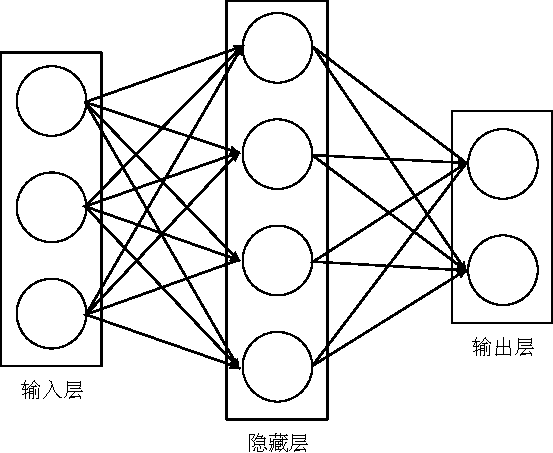
\includegraphics{fc1}
  \caption{全连接神经网络示意图}
  \label{fig:fc1}
\end{figure}

从图中可以看到,全连接神经网络分为多个层,最开始的一层称为输入层,最后面的一层称为输出层,
输入层和输出层之间的其他层称为隐藏层。同一层的神经元之间没有相互连接,相邻两层间的各神经
元之间均相互连接,这也是它被称为全连接神经网络的原因。当然神经网络还有其他很多种连接形式,
比如~\ref{subsection:cnn}节将要介绍的卷积神经网络(Convolutional Neural Network, CNN)等。

\subsubsection{神经网络的计算}

神经网络其实就是一个从输入向量到输出向量的多元非线性函数。由于神经网络是分层的,因此我们
需要从输入向量开始,使用~(\ref{equ:chap3:neuron3})式逐层向前计算,直到输出层的所有神经元计
算完毕为止。以图~\ref{fig:fc2}为例,下面简单给出神经网络的前向计算过程。
\begin{figure}[ht]
  \centering
  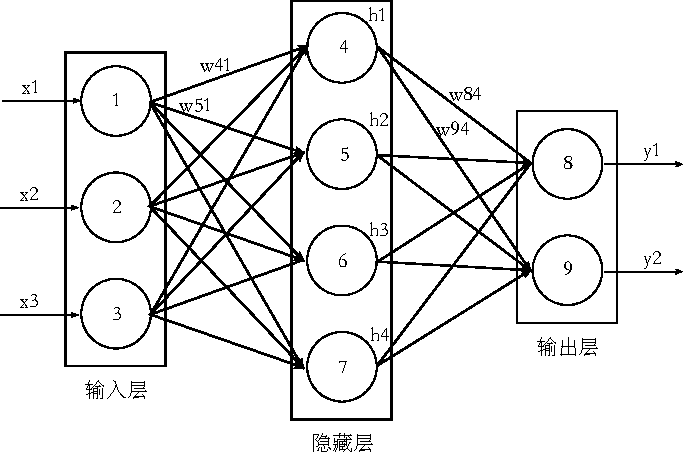
\includegraphics{fc2}
  \caption{神经网络前向计算}
  \label{fig:fc2}
\end{figure}

图中输入层的三个节点分别编号为1、2、3,隐藏层的四个节点分别编号为4、5、6、7,输出层的2个
节点分别编号为8和9。将隐藏层的四个节点处的值组成的向量记为$h=(h_1, h_2, h_3, h_4)^T$,输
入层的节点1和隐藏层的节点4之间连接的权值记为$w_{41}, w_{42}, w_{43}$,那么我们可以得到
$h_1$的计算方法如~(\ref{equ:chap3:cal_hidden})式所示。
\begin{equation}
  \label{equ:chap3:cal_hidden}
  h_1 = f(w^Tx)=f(w_{41}x_1+w_{42}x_2+w_{43}x_3+b_4)
\end{equation}

其中$f(x)$表示激活函数,$b_4$表示偏置项。按照同样的方式,我们可以计算得到$h_2$、$h_3$、
$h_4$。在得到隐藏层所有节点的值之后,我们可以计算输出层节点的值,例如节点8处的值计算方式
如~(\ref{equ:chap3:cal_output})式所示。
\begin{equation}
  \label{equ:chap3:cal_output}
  y_1 = f(w^Th)=f(w_{84}h_1+w_{85}h_2+w_{86}h_3+b_8)
\end{equation}

实际上,上面的计算过程可以写成矩阵乘法的形式,记$x=(x_1,x_2,x_3)^T$,$h=(h_1,h_2,h_3,h_4)^T$,
$y=(y_1,y_2)^T$,那么从输入层到隐藏层的计算过程可以写为:
\begin{equation}
  \label{equ:chap3:matrix_cal_hidden}
  h = f(W\cdot x)
\end{equation}

从隐藏层到输出层的计算过程可以写为:
\begin{equation}
  \label{equ:chap3:matrix_cal_output}
  y = f(W\cdot h)
\end{equation}

\subsubsection{反向传播算法}

设计好一个网络模型后,我们需要在训练样本集上通过大量的迭代计算过程来逐步学习模型的参数,也就是
各层神经元之间连接的权值$w$。神经网络的学习过程一般是通过反向传播算法(Back Propagation, BP)来
完成的。假设训练样本为$(x, d)$,其中向量$x$是训练样本的特征,向量$d$是样本的目标值。在初始化网
络的所有权值之后,首先我们使用上一节中介绍的方式计算各隐藏层的值$h$和输出层的值$y$,然后从输出
层开始,从后向前逐层计算误差项$\delta$。

对于输出层的每个节点,$\delta_i$的计算方式如~(\ref{equ:chap3:delta_i_output})式所示。
\begin{equation}
  \label{equ:chap3:delta_i_output}
  \delta_i = y_i(1-y_i)(d_i-y_i)
\end{equation}

其中,$\delta_i$是节点$i$的误差项,$y_i$是节点$i$的输出值,$d_i$是节点$i$对应的目标值。例如,
对于图~\ref{fig:fc2}中的节点8,$\delta_8$的计算方式如~(\ref{equ:chap3:delta_8})所示。
\begin{equation}
  \label{equ:chap3:delta_8}
  \delta_8 = y_1(1-y_1)(d_1-y_1)
\end{equation}

对于隐藏层中的每个节点,$\delta_i$的计算方式如~(\ref{equ:chap3:delta_i_hidden})式所示。
\begin{equation}
  \label{equ:chap3:delta_i_hidden}
  \delta_i=h_i(1-h_i)\sum_{k\in D(j)}w_{ki}\delta_k
\end{equation}

其中,$D(j)$表示与节点$j$直接相连的所有下游节点,比如在图~\ref{fig:fc2}中节点4的直接下游节点
为节点8和节点9。因此,对于节点4,$\delta_4$的计算方式如~(\ref{equ:chap3:delta_4})式所示。
\begin{equation}
  \label{equ:chap3:delta_4}
  \delta_4=h_1(1-h_1)(w_{84}\delta_8+w_{94}\delta_9)
\end{equation}

最后,我们通过~(\ref{equ:chap3:update_weights})式更新网络中的权值。
\begin{equation}
  \label{equ:chap3:update_weights}
  w_{ji} = w{ji} + \eta \delta_j x_{ji}
\end{equation}

其中,$\eta$是训练过程中设定的一个模型超参数,我们称之为学习速率。计算网络中各节点误差项
以及权值更新的公式在推导过程中本质上都是利用了复合函数的链式求导法则,具体过程本文不再赘述。

\subsection{卷积神经网络}
\label{subsection:cnn}

\subsubsection{ReLU激活函数}

通常情况下卷积神经网络中的激活函数会选择ReLU(Rectified Linear Unit)函数,而不是~\ref{subsection:nn}
中介绍的sigmoid函数,或者tanh函数。~(\ref{equ:chap3:relu})式给出了ReLU函数的定义。
\begin{equation}
  \label{equ:chap3:relu}
  f(x) = \max(0, x)
\end{equation}

图~\ref{fig:relu}给出了ReLU函数的图像。
\begin{figure}[ht]
  \centering
  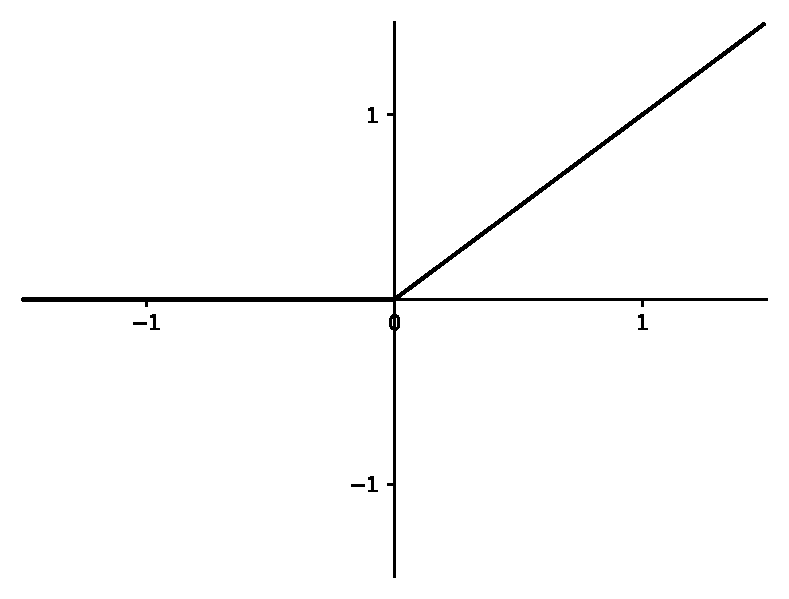
\includegraphics[height=6cm]{relu}
  \caption{ReLU激活函数的图像}
  \label{fig:relu}
\end{figure}

卷积神经网络中通常选择ReLU函数作为激活函数,是因为相对于其他的激活函数,它具有以下两个优点:

1)运算速度快。sigmoid激活函数在计算函数值时,涉及到指数和倒数运算,而ReLU激活函数只涉及到
一个比较运算,计算代价相对要小很多。

2)减轻梯度消失问题。在上一节中我们介绍了通过反向传播算法来训练神经网络,并给出了网络中权值
的更新公~(\ref{equ:chap3:update_weights})式,以及误差项的计算公~(\ref{equ:chap3:delta_i_output})式
和~(\ref{equ:chap3:delta_i_hidden})。从误差项$\delta$的计算公式可以看出,计算$\delta$的时候
总是要乘以sigmoid函数的导数值$\sigma^\prime$。从图~\ref{fig:derivative_sigmoid}中可以看出,
$\sigma^\prime$的取值范围为$(0, 1/4]$,那么从后向前逐层计算的过程中,误差项将会越来越小,
也就是梯度会越来越小,这在深层的网络结构中对于更新网络权值非常不利。而ReLU激活函数的导数值
为1,因此不会导致这个问题。
\begin{figure}[ht]
  \centering
  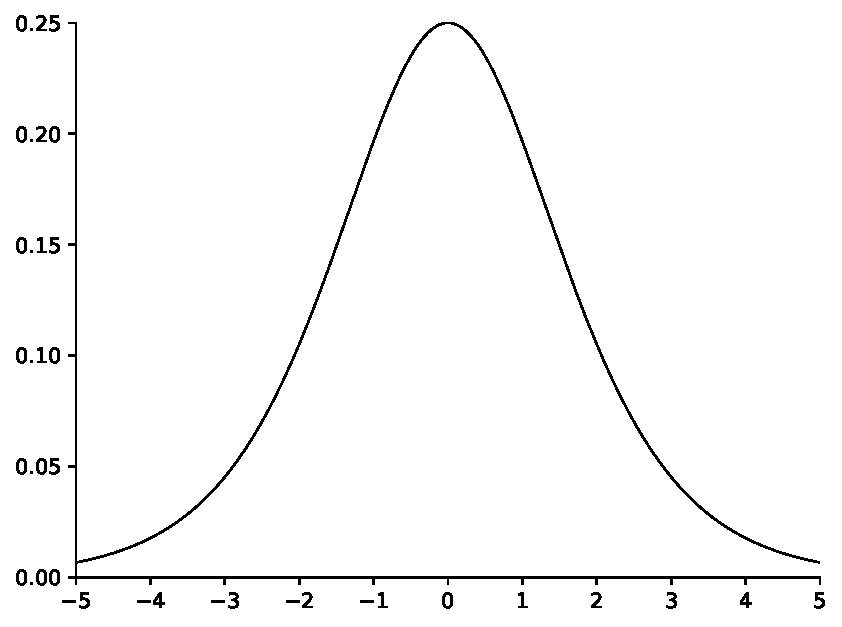
\includegraphics[height=6cm]{derivative_sigmoid}
  \caption{sigmoid导函数图像}
  \label{fig:derivative_sigmoid}
\end{figure}

\subsubsection{网络结构}

卷积神经网络和~\ref{subsection:nn}节中介绍的一般的神经网络结构非常相似。它们都是由大量带有
权值向量的神经元构成,每个神经元接受一些输入值,与权值向量做内积,然后对结果施加一个非线性
激活函数。整个网络同样有一个可导的目标函数,我们同样可以通过反向传播的方式来学习网络中的权
值。但是卷积神经网络改变了相邻两层神经元之间的连接方式,同时引入了权值共享的设定,从而极大
程度地降低了网络中权值的个数,使得网络的规模能够进一步地扩展。

首先我们来说明常规的神经网络结构在构建大规模网络时的局限。假设网络的输入是$200\times 200 
\times 3$的图像(宽度和高度均为200个像素,3个颜色通道),如果采用全联接的方式,那么第一个
隐藏层中的一个节点就会有$200\times 200\times 3=12000$个权值。当然,通常情况下每个隐藏层都
会有多个节点,而且网络中也不止有一个隐藏层,因此网络中的权值会随着网络规模的增大而急剧增加。
很明显这种全联接的网络结构会导致大量网络参数的浪费,并且很容易造成模型的过拟合。

CNN最初是针对解决图像问题而设计的,图片中的像素是排列在3个维度(宽度、高度和颜色通道)上的,
因此CNN在组建网络结构的时候仿照了图片像素的这种排列方式,即每一层的所有节点均排列为3个维度
(宽度、高度和深度)。例如对于CIFAR-10数据集中的图片,网络输入层的维度将是$32\times 32\times3$。
某一层中的节点将不再与前一层的所有节点连接,而是仅与前一层中一个较小区域中的节点连接,我们
称之为局部连接方式,本节后面部分会详细介绍。对于CIFAR-10数据集,由于这是一个10种类别的分类
问题,因此网络最后的输出层维度是$1\times 1\times 10$。图~\ref{fig:cnn}是CNN中节点排列方式
的示意图。
\begin{figure}[ht]
  \centering%
  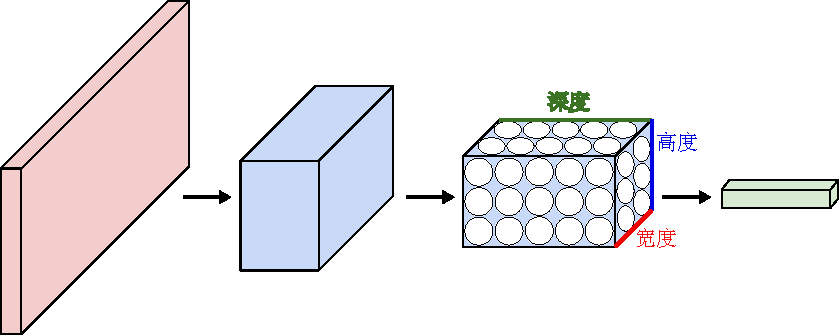
\includegraphics{cnn}
  \caption{CNN中节点排列方式示意图}
  \label{fig:cnn}
\end{figure}

从图中可以看出,一个简单的卷积神经网络由顺序排列的多个层(Layer)组成,每一层的所有节点都
排列在宽度、高度和深度3个维度上,形成一个立方体的形状,我们将排列成这种立方体形状的一层节
点称为一个特征图(Feature Map)。相邻两层特征图之间通过一个可导函数变换得到,不同的变换方
式对应着不同类型的层。最常用的一些层有:卷积层(Convolutional Layer)、下采样层(Pooling
 Layer)和全连接层(Fully Connected Layer)。我们将这些层按照一定的次序堆叠在一起就构成了
 卷积神经网络。图~\ref{fig:cnn_typical}是包含这三种层的一个典型的卷积神经网络结构。
\begin{figure}[ht]
  \centering%
  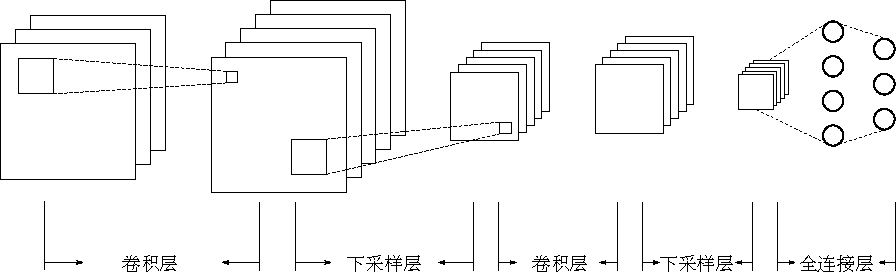
\includegraphics{cnn_typical}
  \caption{典型的CNN结构}
  \label{fig:cnn_typical}
\end{figure}

下面我们逐个介绍各个层。

1)卷积层

卷积层的参数由一组可学习的卷积核(Filter)组成。通常卷积核在空间上的尺寸(宽度和高度)比较小,
深度和上一层的深度相同。例如在图~\ref{fig:cnn_typical}中,第一个卷积层中的卷积核尺寸可以是
$5\times 5\times 3$(宽度方向和高度方向各5个像素,深度与图片通道数相等,等于3)。此外,卷积
核的个数决定了下一层特征图的深度,例如图~\ref{fig:cnn_typical}中第一个卷积层的卷积核个数为5。
各卷积核与上一层特征图沿着宽度和高度方向进行卷积运算,对运算得到的结果施加ReLU激活函数,并且
将所有卷积核对应的结果按深度方向排列在一起,即可得到下一层的特征图。图~\ref{fig:convolve}展示
了一个$3\times 3\times 3$的卷积核与$5\times 5\times 3$的特征图间的卷积运算。
\begin{figure}[ht]
  \centering%
  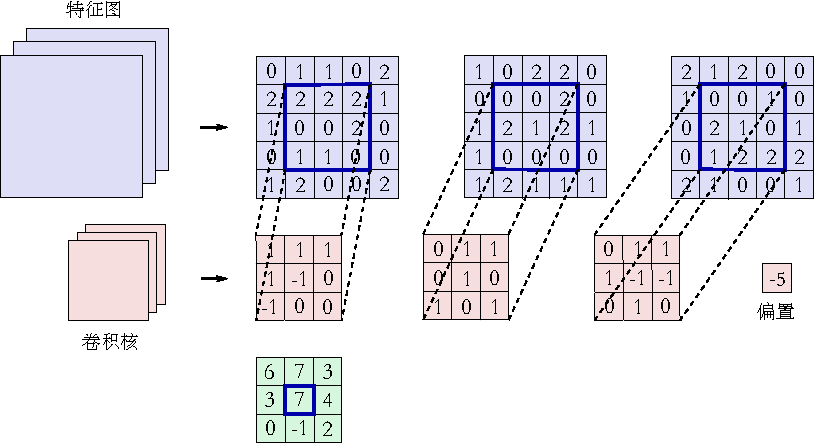
\includegraphics{convolve}
  \caption{卷积核与特征图间的卷积运算}
  \label{fig:convolve}
\end{figure}

从图中可以看出,在卷积核与特征图之间做卷积运算时,下一层特征图中的节点只和上一层中与卷积核
尺寸相同数目的节点相连接,而不是与所有节点连接,这种局部连接的方式能够在很大程度上降低网络
中权值的个数。例如对于图~\ref{fig:convolve}中的卷积运算,下一层特征图中的节点只需要与上一层
中的$3\times 3\times 3=27$个节点相连。

图~\ref{fig:convolve}展示的卷积运算过程中,步长(Stride)为1,也就是卷积核在空间方向上移动的
长度,步长也可以取其他大于1的正整数值。此外,从图中我们可以发现,经过卷积层之后,特征图在空间
上的尺寸由$5\times5$变成了$3\times 3$。很多时候,我们不希望卷积层改变特征图在空间上的尺寸,
因为这会丢失一些边缘信息。我们可以通过在边界四周补0(Zero Padding)的方式得到空间上尺寸不变的
结果,如图~\ref{fig:padding}所示。
\begin{figure}[ht]
  \centering%
  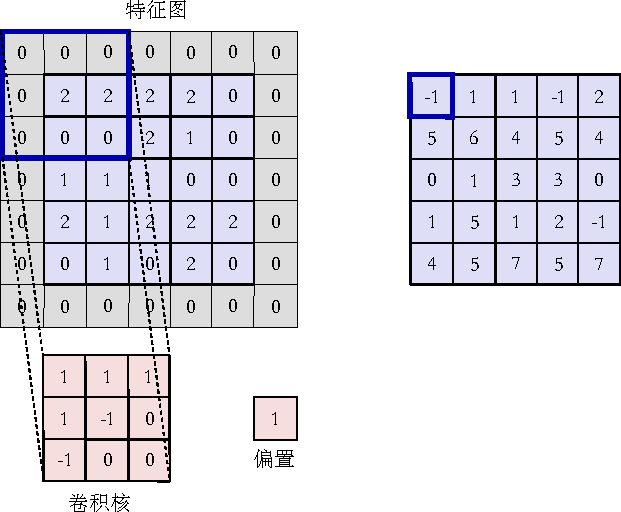
\includegraphics{padding}
  \caption{卷积过程中补零操作示意图}
  \label{fig:padding}
\end{figure}

一般地,如果卷积层输入的特征维度为$W_1\times H_1 \times D_1$,卷积核个数为$K$,卷积核在空间上
的尺寸为$F$,步长为$S$,边界四周补零的圈数为$P$,输出的特征图维度为$W_2\times H_2\times D_2$,
那么有:
\begin{equation}
  \label{equ:chap3:conv_dim}
  \left\{\begin{aligned}
    & W_2 = (W_1 - F + 2P)/S + 1 \\
    & H_2 = (H_1 - F + 2P)/S + 1 \\
    & D_2 = K
  \end{aligned}\right.
\end{equation}

因此,卷积层向网络中引入了$(F\cdot F\cdot D_1)\cdot K$个权值参数,以及$K$个偏置参数。

2)下采样层

在卷积神经网络中,通常会在连续的多个卷积层之间加入一个下采样层,它的作用在于逐步降低特征图
在空间上的尺寸,从而减少网络中的参数数量和计算量,因此能够在一定程度上防止过拟合。与卷积操作
不同,下采样层独立操作深度方向上的每一个切片,用最大值操作来对每个切片在空间上的尺寸进行压缩。
最常见的形式是核宽度为$2\times 2$、步长为2的下采样层,它可以减少75\%的特征个数。下采样层不改变
特征图的深度。图~\ref{fig:max_pooling}是最大值下采样作用于单个切片上的示意图。
\begin{figure}[ht]
  \centering%
  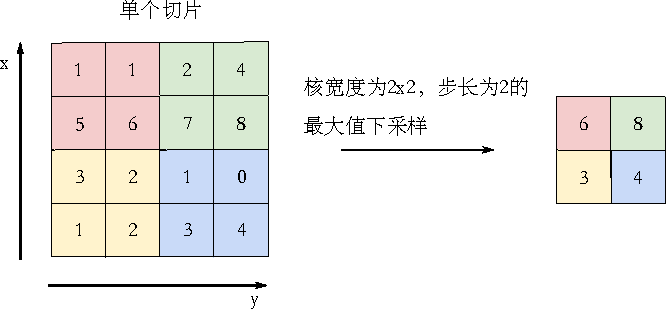
\includegraphics{max_pooling}
  \caption{单个切片上最大值下采样示意图}
  \label{fig:max_pooling}
\end{figure}

一般地,如果下采样层输入的特征图维度为$W_1\times H_1\times D_1$,核宽度为$F$,步长为$S$,输出
的特征图维度为$W_2\times H_2\times D_2$,那么有:
\begin{equation}
  \label{equ:chap3:pool_dim}
  \left\{\begin{aligned}
    & W_2 = (W_1 - F)/S + 1 \\
    & H_2 = (H_1 - F)/S + 1 \\
    & D_2 = D_1
  \end{aligned}\right.
\end{equation}

通常情况下,除了最大值下采样(Max Pooling),常见的下采样层还有平均值下采样(Average Pooling)
和L2-norm下采样。无论是哪一类下采样层,都不会向网络中引入参数。

3)全连接层

和一般的神经网络中神经元的连接方式一样,全连接层中的节点与前一层中的所有节点相连接。这一部分
在~\ref{subsection:nn}节中有详细介绍,此处不再赘述。

\section{基于卷积神经网络的故障诊断模型}

第~\ref{cha:chapter2}章中使用单层的平均值下采样对信号的频谱序列进行了特征提取,取得了不错的
效果。因此在介绍本章基于CNN的故障诊断模型之前,我们首先来验证CNN中更常用的最大值下采样从信号
的频谱序列中提取特征的效果。

同样,给定一个信号片段$x$,假设其采样点数为$N$,即$x = (x_1,x_2,...,x_N)^T$,下采样的核宽度
为$F$,下采样步长$S=F$。由~\ref{subsection:cnn}中的介绍可知,下采样之后的特征向量长度
$L = (N-F)/S+1=N/F$。与第二章中一样,我们首先对$x$做实数形式的傅立叶变换,得到$x$的RDFT频谱
序列$\widetilde{x} = (\widetilde{x}_1, \widetilde{x}_2, ..., \widetilde{x}_N)^T$。同样,为了避免样本相位的不一致对
最终模型的诊断精度产生影响,同时也避免在后续的操作中正负值相互抵消,我们对$\widetilde{x}$取了绝对
值,即$X = (|\widetilde{x}_1|, |\widetilde{x}_2|, ..., |\widetilde{x}_N|)^T$。下采样之后得到的特征向量记为
$V = (V_1, V_2, ..., V_L)^T$,那么参考平均值下采样的计算式~(\ref{equ:chap2:pooling}),最大值
下采样可以写为~(\ref{equ:chap3:max_pooling})式。
\begin{equation}
  \label{equ:chap3:max_pooling}
  V_k = \max_{j=1,...,F}X_{(k-1)F+j}, k=1,2,...,L
\end{equation}

图~\ref{fig:average_max_pooling_features}是某个采样点数为384的信号片段的原始波形、其对应的RDFT频谱序列、以及
分别使用平均值下采样和最大值下采样提取的维度为32的特征向量。
\begin{figure}[ht]
  \centering
  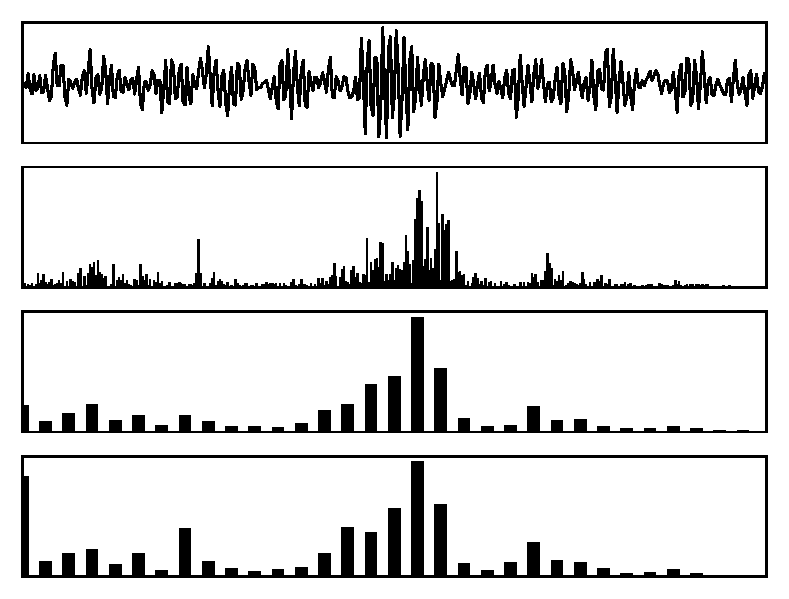
\includegraphics[height=8cm]{average_max_pooling_features}
  \caption{平均值下采样和最大值下采样提取的特征向量}
  \label{fig:average_max_pooling_features}
\end{figure}

从图中可以看出,使用最大值下采样在信号频谱上提取的特征跟使用平均值下采样获得的结果是类似的。
接下来我们用最大值下采样提取的特征训练并测试第~\ref{cha:chapter2}章中设计的故障诊断模型,在
这过程中,保持模型中的超参数设置不变,即SVM算法的惩罚因子$C=1$,高斯核宽度参数$\sigma=L$。
分别取特征个数$L$为3、6、12、24、48、96、192,对应下采样核宽度$F$为128、64、32、16、8、4、2,
依次训练并测试分类模型。与第~\ref{cha:chapter2}章中得到的结果类似,在特征个数$L=48$即下采样
核宽度$F=8$时,模型预测精度达到最高,为94.23\%。

在卷积神经网络中,我们通常会堆叠多层卷积层和下采样层,这样的结构优势在于能够逐层地提取并筛选
特征,从而得到更加高级和抽象的特征。图~\ref{fig:convnet}展示了CIFAR-10数据集上的一个CNN分类
模型的各层特征图。
\begin{figure}[ht]
  \centering%
  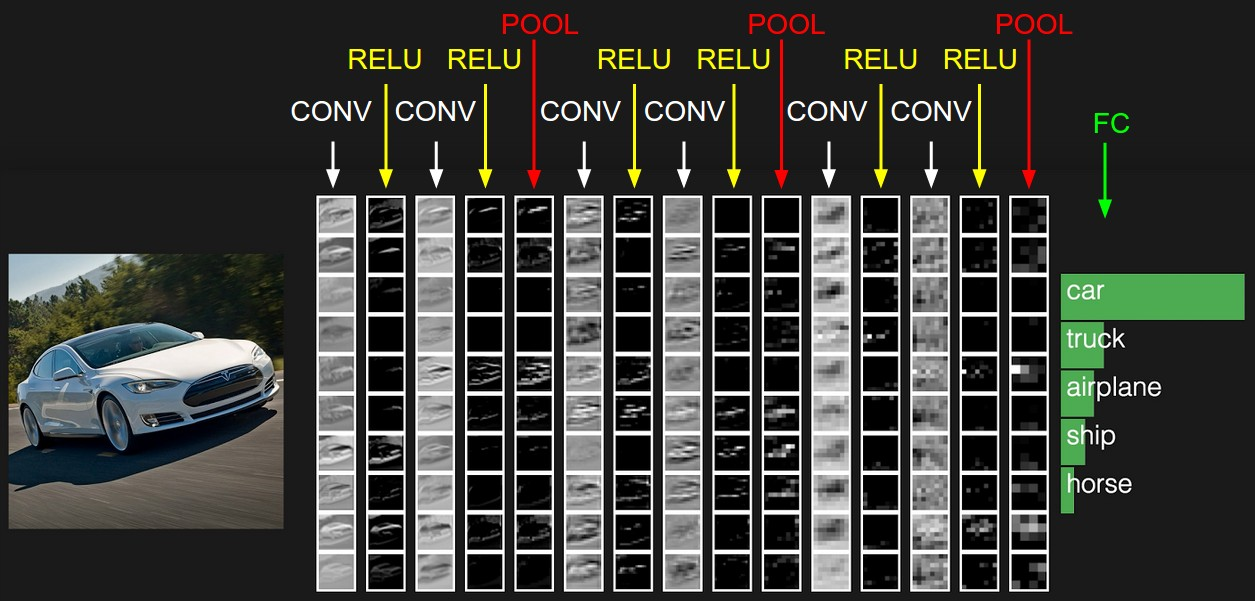
\includegraphics[width=13cm]{convnet}
  \caption{CNN模型各层特征图可视化结果示例}
  \label{fig:convnet}
\end{figure}

图~\ref{fig:convnet}中最左边是网络的输入,也就是原始图片,最右边输出对应图片的类别信息。图中
从左至右的每一列分别是网络中每一层输出的特征图。由于3维的特征图不容易显示,因此图中将特征图
沿深度方向的所有切片显示成一列。可以看出网络中最开始的几层主要是提取一些底层特征,例如图片中
的纹理、边缘、明暗等特征;网络中越后面的层提取的特征就越高级和抽象,更能反映出图片的类别信息。
因此可以说CNN网络在原始输入上提取特征的过程是逐层抽象的过程,比直接使用单层下采样提取特征的过
程显然更加合理,提取到的特征也势必更能反映类别信息。鉴于此,本章设计了一个结构与VGG类似的故障
诊断模型,如图~\ref{fig:cnn_classifier}所示。
\begin{figure}[ht]
  \centering%
  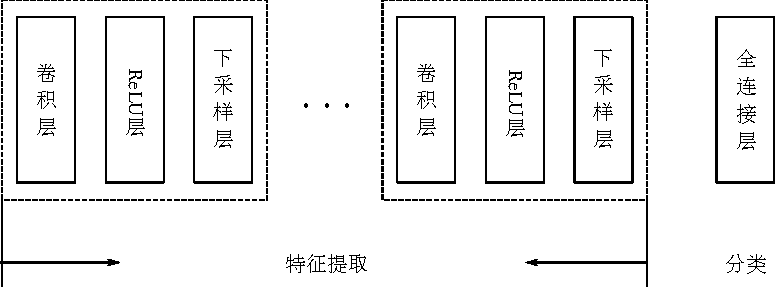
\includegraphics{cnn_classifier}
  \caption{基于CNN的故障诊断模型示意图}
  \label{fig:cnn_classifier}
\end{figure}

图~\ref{fig:cnn_classifier}中特征提取阶段基本构成单元为顺序相连的一个卷积层、一个非线性激活
层和一个下采样层,如图中虚线框所示。根据情况我们可以连续堆叠多个这样的单元来完成我们的特征提取
过程。在网络的最后,我们使用一个全连接层对提取的特征进行分类。

与第~\ref{cha:chapter2}不同,本章的特征提取和分类过程不是独立进行的,而是由同一个网络实现的。
因此,提取的特征也能够更好地反映输入数据和类别标签之间的关系。此外,特征提取环节存在大量的网络
参数可以学习,在一定程度上讲,这个模型中的特征提取方式是学习出来的,而不是直接指定的,从而能够
提取输入的信号频谱中更加本质的特征。

由于网络的输入是一维的信号频谱序列,因此我们的模型中用到的卷积层和下采样层都是沿着一维方向
进行的。图~\ref{fig:convolve_1d}是一维方向卷积操作的示例。
\begin{figure}[ht]
  \centering%
  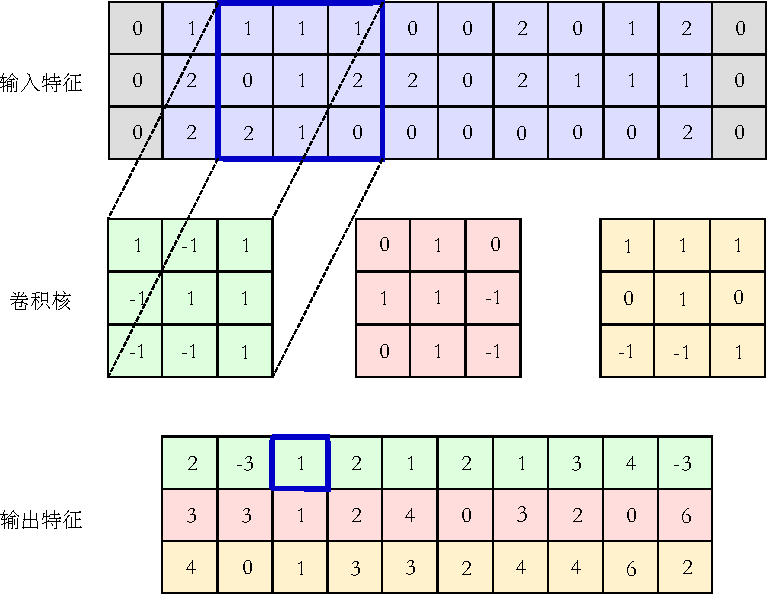
\includegraphics{convolve_1d}
  \caption{一维方向卷积操作示例}
  \label{fig:convolve_1d}
\end{figure}

图~\ref{fig:convolve_1d}中输入是维度为$3\times10$的特征图,与3个$3\times 3$的卷积核
进行一维的卷积操作后,输出维度为$3\times 10$的特征图。可以看出,一维方向的卷积操作
相当于二维情况下宽度或高度为1时的退化结果。

\section{仿真实验}

\subsection{实验过程}

在本章的仿真实验中,我们使用5个图~\ref{fig:cnn_classifier}中虚线框表示的基本单元顺序连接,
各层节点的数据维度变化情况如图~\ref{fig:cnn_data}所示。图中的模块1-5均表示卷积层+ReLU层
+下采样层的结构,各模块中的卷积层和下采样层的参数如表~\ref{tab:layer_parameters}所示。
\begin{figure}[ht]
  \centering%
  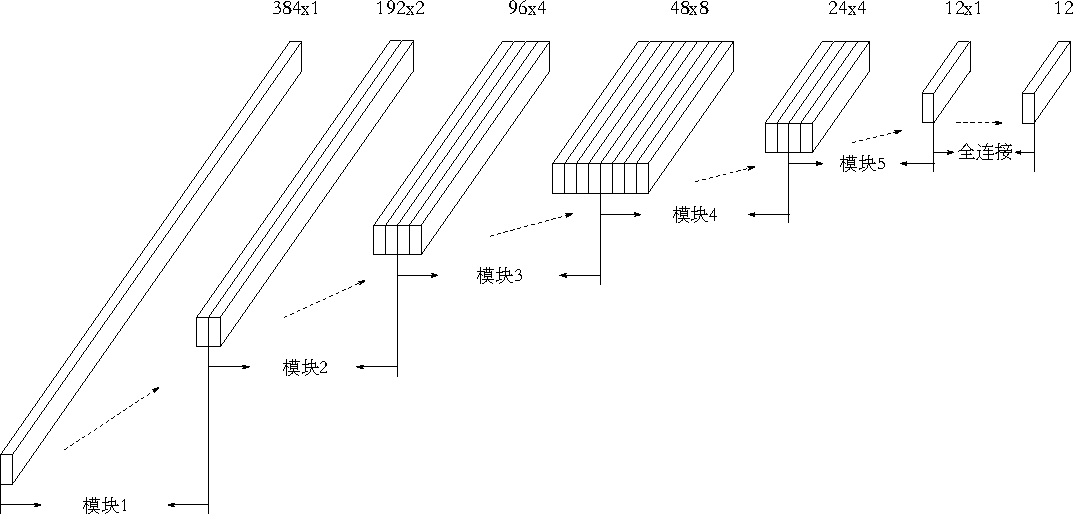
\includegraphics[width=14cm]{cnn_data}
  \caption{模型各层数据维度变化情况}
  \label{fig:cnn_data}
\end{figure}

\begin{table}[htb]
  \centering
  \begin{minipage}[t]{0.8\linewidth} % 如果想在表格中使用脚注,minipage是个不错的办法
  \caption{模型各层结构参数列表}
  \label{tab:layer_parameters}
    \begin{tabularx}{\linewidth}{lXXX}
      \toprule[1.5pt]
      网络模块 & 卷积核宽度 & 卷积核个数 & 下采样核宽度 \\\midrule[1pt]
      模块1 & 3 & 2 & 2 \\
      模块2 & 3 & 4 & 2 \\
      模块3 & 3 & 8 & 2 \\
      模块4 & 3 & 4 & 2 \\
      模块5 & 3 & 1 & 2 \\
      \bottomrule[1.5pt]
    \end{tabularx}
  \end{minipage}
\end{table}

图中网络的输入是信号片段对应的频谱序列$X$,维度为384。由于第一个模块的卷积核个数为2,
下采样核宽度为2,因此经过第一个模块后,网络中的特征图维度变为$192\times 2$;同理,经
过第二个模块后,网络中特征图的维度变为$96\times 4$;经过第三个模块后,网络中特征图的
维度变为$48\times 8$;经过第四个模块后,网络中特征图的维度变为$24\times 4$;经过第五
个模块后,网络中特征图的维度变为$12\times 1$。这个长度为12的向量就是我们的网络从原始
信号频谱序列中提取的特征向量,后面再连接一个全连接层进行故障分类。

\subsection{实验结果及分析}

网络训练好之后,我们从测试集的每一类样本中随机选择3个信号片段,分别计算其RDFT频谱序列,
并将其输入到网络中,得到网络提取的特征向量,如图~\ref{fig:cnn_features}所示。
\begin{figure}[ht]
  \centering%
  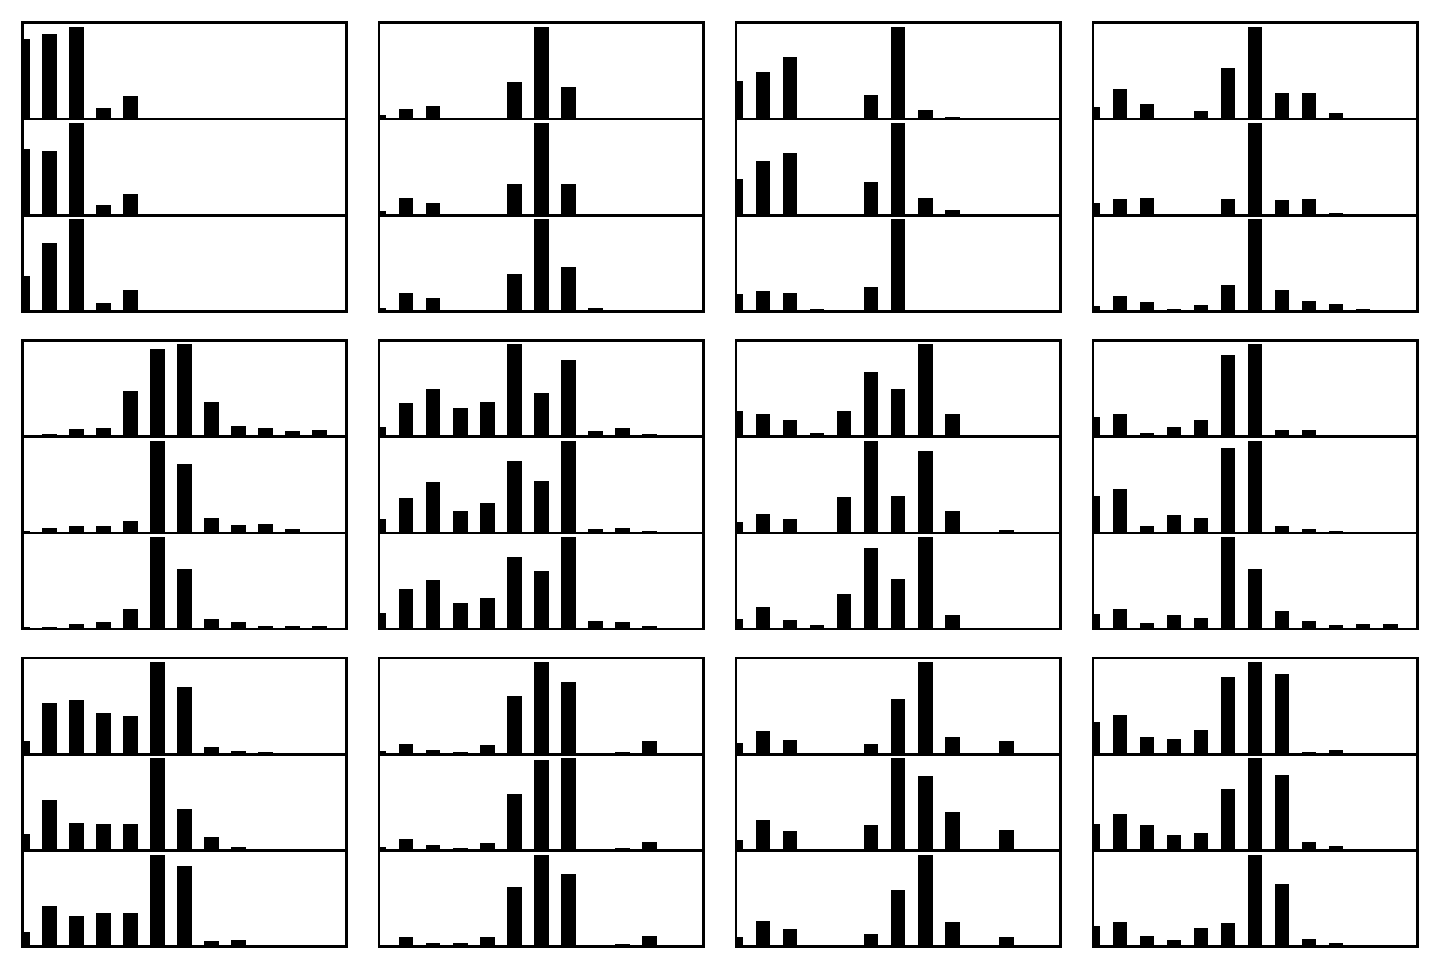
\includegraphics[height=9cm]{cnn_features}
  \caption{CNN模型提取的特征向量}
  \label{fig:cnn_features}
\end{figure}

可以看出,与图~\ref{fig:average_pooling_features_12}中显示的使用单层平均值下采样提取的
特征向量相比,使用本章中的特征提取方法获得的结果在类别之间具有更好的区分性,而同一类样
本之间的相似程度也更高。最后本章的故障诊断模型可以达到98.27\%的预测精度,也印证了这一点。
但是,本章模型的训练时间为102s,远高于第~\ref{cha:chapter2}章中基于SVM的级联分类模型训练
所用时间,这也是基于CNN的模型的缺点之一。表~\ref{tab:chap3:confusion_matrix}给出了模型在
测试集上的混淆矩阵。
\begin{table}[htb]
  \centering
  \begin{minipage}[t]{0.9\linewidth} % 如果想在表格中使用脚注,minipage是个不错的办法
  \caption{基于CNN的故障诊断模型在测试集上的混淆矩阵}
  \label{tab:chap3:confusion_matrix}
    \begin{tabularx}{\linewidth}{l|XXXXXXXXXXXX}
      \toprule[1.5pt]
         0 &   1 &   2 &   3 &   4 &   5 &   6 &   7 &   8 &   9 &  10 &  11 \\\midrule[1pt]
      1579 &   0 &   0 &   0 &   0 &   0 &   0 &   0 &   0 &   0 &   0 &   0 \\
         0 & 697 &   2 &  11 &   0 &   0 &   0 &   0 &   0 &   0 &   0 &   0 \\
         0 &  83 & 682 &  18 &   0 &   0 &   0 &   0 &   0 &   0 &   0 &   1 \\
         0 &  20 &   0 & 765 &   0 &   0 &   0 &   0 &   0 &   0 &   0 &   0 \\
         0 &   0 &   0 &   0 & 777 &   0 &   0 &   0 &   0 &   0 &   0 &   0 \\
         0 &   0 &   0 &   0 &   0 & 780 &   0 &   0 &   0 &   0 &   0 &   0 \\
         0 &   0 &   0 &   0 &   0 &   0 & 784 &   0 &   0 &   0 &   0 &   0 \\
         0 &   0 &   0 &   0 &   0 &   0 &   0 & 786 &   0 &   0 &   0 &   0 \\
         0 &   0 &   0 &   0 &   0 &   0 &   0 &   0 & 777 &   0 &   0 &   0 \\
         0 &   0 &   0 &   0 &   0 &   0 &   0 &   0 &   0 & 785 &   0 &   0 \\
         0 &   0 &   0 &   0 &   0 &   0 &   0 &   0 &   0 &   0 & 784 &   0 \\
         0 &   0 &   0 &   0 & 195 &   0 &   1 &   2 &   0 &  56 &   0 & 534 \\
      \bottomrule[1.5pt]
    \end{tabularx}
  \end{minipage}
\end{table}

\section{小结}

本章对神经网络做了简单的介绍,然后介绍了卷积神经网络的结构,并且基于CNN提出了一种适用
与故障诊断领域的模型,实现了对信号片段的特征提取和故障模式分类。本章设计的模型提取的
特征向量维度为12,能够在测试集上达到的预测精度为98.27\%,这与第~\ref{cha:chapter2}章
中得到的93.81\%的预测精度相比,已经有了很大的提升。此外,第~\ref{cha:chapter2}章中的
模型达到93.81\%的最佳预测精度时,提取的特征向量的维度$L=48$,特征个数相当于本章中特征
个数的4倍。从表~\ref{tab:chap2_acc_time}可以看到,当第~\ref{cha:chapter2}章中的模型取
特征维度$L=12$时,模型预测精度只能达到87.84\%。由此可见,本章中基于CNN的故障特征提取
及分类模型是非常有效的。



%%% 其它部分
\backmatter

%% 参考文献
% 注意:至少需要引用一篇参考文献,否则下面两行可能引起编译错误。
% 如果不需要参考文献,请将下面两行删除或注释掉。
\bibliographystyle{thuthesis}
\bibliography{ref/refs}


%% 致谢
% 如果使用声明扫描页,将可选参数指定为扫描后的 PDF 文件名,例如:
% \begin{acknowledgement}[scan-statement.pdf]
\begin{acknowledgement}
  衷心感谢导师 xxx 教授和物理系 xxx 副教授对本人的精心指导。他们的言传身教将使
  我终生受益。

  在美国麻省理工学院化学系进行九个月的合作研究期间,承蒙 xxx 教授热心指导与帮助,不
  胜感激。感谢 xx 实验室主任 xx 教授,以及实验室全体老师和同学们的热情帮助和支
  持!本课题承蒙国家自然科学基金资助,特此致谢。

  感谢 \thuthesis,它的存在让我的论文写作轻松自在了许多,让我的论文格式规整漂亮了
  许多。
\end{acknowledgement}


%% 个人简历
\begin{resume}

  \resumeitem{个人简历}

  xxxx 年 xx 月 xx 日出生于 xx 省 xx 县。

  xxxx 年 9 月考入 xx 大学 xx 系 xx 专业,xxxx 年 7 月本科毕业并获得 xx 学士学位。

  xxxx 年 9 月免试进入 xx 大学 xx 系攻读 xx 学位至今。

  \researchitem{发表的学术论文} % 发表的和录用的合在一起

  % 1. 已经刊载的学术论文(本人是第一作者,或者导师为第一作者本人是第二作者)
  \begin{publications}
    \item Yang Y, Ren T L, Zhang L T, et al. Miniature microphone with silicon-
      based ferroelectric thin films. Integrated Ferroelectrics, 2003,
      52:229-235. (SCI 收录, 检索号:758FZ.)
    \item 杨轶, 张宁欣, 任天令, 等. 硅基铁电微声学器件中薄膜残余应力的研究. 中国机
      械工程, 2005, 16(14):1289-1291. (EI 收录, 检索号:0534931 2907.)
    \item 杨轶, 张宁欣, 任天令, 等. 集成铁电器件中的关键工艺研究. 仪器仪表学报,
      2003, 24(S4):192-193. (EI 源刊.)
  \end{publications}

  % 2. 尚未刊载,但已经接到正式录用函的学术论文(本人为第一作者,或者
  %    导师为第一作者本人是第二作者)。
  \begin{publications}[before=\publicationskip,after=\publicationskip]
    \item Yang Y, Ren T L, Zhu Y P, et al. PMUTs for handwriting recognition. In
      press. (已被 Integrated Ferroelectrics 录用. SCI 源刊.)
  \end{publications}

  % 3. 其他学术论文。可列出除上述两种情况以外的其他学术论文,但必须是
  %    已经刊载或者收到正式录用函的论文。
  \begin{publications}
    \item Wu X M, Yang Y, Cai J, et al. Measurements of ferroelectric MEMS
      microphones. Integrated Ferroelectrics, 2005, 69:417-429. (SCI 收录, 检索号
      :896KM)
    \item 贾泽, 杨轶, 陈兢, 等. 用于压电和电容微麦克风的体硅腐蚀相关研究. 压电与声
      光, 2006, 28(1):117-119. (EI 收录, 检索号:06129773469)
    \item 伍晓明, 杨轶, 张宁欣, 等. 基于MEMS技术的集成铁电硅微麦克风. 中国集成电路,
      2003, 53:59-61.
  \end{publications}

  \researchitem{研究成果} % 有就写,没有就删除
  \begin{achievements}
    \item 任天令, 杨轶, 朱一平, 等. 硅基铁电微声学传感器畴极化区域控制和电极连接的
      方法: 中国, CN1602118A. (中国专利公开号)
    \item Ren T L, Yang Y, Zhu Y P, et al. Piezoelectric micro acoustic sensor
      based on ferroelectric materials: USA, No.11/215, 102. (美国发明专利申请号)
  \end{achievements}

\end{resume}


\end{document}
